%%%%%%%%%%%%%%%%%%%%%%%%%%%%%%%%%%%%%%%%%%%%%%%%%%%%%%%%%%%%%%%%%%%%%%%%%%%
%% Rulebook RoboCup Logistics League Sponsored by Festo
%% 2015 Competitions
%%%%%%%%%%%%%%%%%%%%%%%%%%%%%%%%%%%%%%%%%%%%%%%%%%%%%%%%%%%%%%%%%%%%%%%%%%%

\documentclass[12pt,twoside]{article}

\usepackage[a4paper]{anysize}
\marginsize{2cm}{2cm}{1cm}{2cm}

\setlength{\marginparwidth}{1cm}
%\usepackage{fourier}
%\newcommand\rulechange[1]{\begin{shaded}#1\end{shaded}\marginpar{\LARGE\danger}}

%% MACROS %%%%%%%%%%%%%%%%%%%

% does not work for me, gives:
%! Undefined control sequence.
%\@ympar ...lobal \setbox \@currbox \copy \@marbox 
%                                                  \@xympar 
%\newenvironment{rulechange}{%
%  \def\FrameCommand{\fboxsep=\FrameSep \colorbox{shadecolor}}%
%  \marginpar{\vspace*{2em}\LARGE\danger} \MakeFramed  {\FrameRestore}}%
% { \endMakeFramed}
\newenvironment{rulechange}{}{}

\usepackage[binary-units=true]{siunitx}

%\usepackage{framed,xcolor}
%\colorlet{shadecolor}{gray!25}
%\textregistered
\newcommand{\Robotino}{Robotino}
\newcolumntype{R}{>{\raggedleft\arraybackslash}X}
\newcolumntype{C}{>{\centering\arraybackslash}X}

\newsavebox{\myt}
\newcommand{\mytable}[1]{\savebox{\myt}{#1}\tikz\node[fill=gray!25!white]{\usebox{\myt}};}

\newcommand{\refsec}[1]{Section~\ref{#1}}
\newcommand{\reffig}[1]{Figure~\ref{#1}}
\newcommand{\refdef}[1]{Definition~\ref{#1}}
%\newcommand{\reflst}[1]{Listing~\ref{#1}}
\newcommand{\reflst}[1]{Figure~\ref{#1}}
\newcommand{\reftab}[1]{Table~\ref{#1}}

\usepackage{floatrow}
\newfloatcommand{capbtabbox}{table}[][\FBwidth]


%% GRAPHICSX %%%%%%%%%%%%%%%%%%%
\usepackage[pdftex]{graphicx}
\graphicspath{{figures/}}
\DeclareGraphicsExtensions{.pdf,.jpeg,.png,.JPG,.jpg}

%% TIKZ %%%%%%%%%%%%%%%%%%%
\usepackage{tikz}
\usetikzlibrary{arrows,shadows}
\usetikzlibrary{calc,positioning}
\usetikzlibrary{snakes,shapes}
\usetikzlibrary{shapes.callouts}

%% HYPERREF %%%%%%%%%%%%%%%%%%%
\usepackage{hyperref}
\hypersetup{
  pdftitle      = {The RoboCup Logistics League Rulebook for 2015},
  pdfauthor     = {RCLL TC},
  pdfkeywords   = {RCLL, Rulebook},
  pdfsubject    = {},
  %pdfpagemode   = {UseOutlines},        % PageWdth, FullScreen, None ...
  hidelinks    = true,          % true colored links, false colored boxes
%  linkcolor     = black,
%  citecolor     = black,
%  filecolor     = black,
%  urlcolor      = black,
%  backref       = false,
%  pagecolor     = black,         % link to other document pages
%  linktocpage,                  % linked page numbers instead of titles
%  menucolor   = blue,           % Acrobat menu item
%  pdfnewwindow= true,                %
%  pdfborder   = {0 0 0},             %
%  bookmarksopen=true,                %
%  bookmarksnumbered=true,            %
%  pdfcreator   = {pdflatex},
%  pdfproducer  = {latex-pdftex}
}

%% SVN-MULTI %%%%%%%%%%%%%%%%%%%
%\usepackage{svn-multi}

%% TODONOTES %%%%%%%%%%%%%%%%%%%
\usepackage{todonotes}

%% TIMES  %%%%%%%%%%%%%%%%%%%
\usepackage{times}

%% TABLES %%%%%%%%%%%%%%%%%%%
\usepackage{tabularx}
\usepackage{multicol}
\usepackage{multirow}
\usepackage{calc}
\usepackage{float}
\restylefloat{table}

\usepackage[TABBOTCAP]{subfigure}
%% INPUTENC %%%%%%%%%%%%%%%%%%%
\usepackage{wasysym}
\usepackage[utf8]{inputenc}
%%%%%%%%%%%%%%%%%%%%%%%%%%%%%%%%%%%%%%%%%%%%%%%%%%%%%%%%%%%%%%%%%%%%%%%%%%%%%
%%% Ruebook RoboCup Logistics League Sponsored by Festo 
%%% Draft for 2013 Competition
%%%%%%%%%%%%%%%%%%%%%%%%%%%%%%%%%%%%%%%%%%%%%%%%%%%%%%%%%%%%%%%%%%%%%%%%%%%%%


\newcommand{\s}[1]{\ensuremath{S_{#1}}}
\newcommand{\p}[1]{\ensuremath{P_{#1}}}
\newcommand{\m}[1]{\ensuremath{M_{#1}}}
\newcommand{\T}[1]{\ensuremath{T_{#1}}}
\newcommand{\dg}[1]{\ensuremath{DG_{#1}}}
\newcommand{\TAG}[1]{\texttt{#1}}


\usepackage[style=numeric,backend=bibtex,maxbibnames=10]{biblatex}
\addbibresource{rulebook2015}


\begin{document}

%%%%%%%%%%%%%%%%%%%%%%%%%%%%%%%%%%%%%%%%%%%%%%%%%%%%%%%%%%%%%%%%%%%%%%%%%%%%%
%%% Titlepage
\hypersetup{pageanchor=false}
\pagenumbering{roman}


\begin{titlepage}
  \vspace*{5cm}
  \begin{center}
    \begin{LARGE}
      
      {\bf RoboCup Logistics League}\\[2ex]
      {\Large Rules and Regulations 2015}\\[4ex]
    \end{LARGE}
    \hrule
    
    {\LARGE\vspace*{4ex}}
    \begin{Large}
      The Technical Committee 2012--2015\\[6ex]
    \end{Large}
    \begin{tabular}{lll}
    \emph{Christian Deppe}&Daniel Ewert&Nils Harder\\
    \emph{S\"oren Jentzsch}&Nicolas Meier&\emph{Tim Niemueller}\\
      Sebastian Reuter&\emph{Alain Rohr}&\emph{Wataru Uemura}\\
    \end{tabular}
    \vfill
    Revision Date: DRAFT -- Work in Progress %February 21\textsuperscript{\raisebox{-.2ex}{st}} 2015
  \end{center}
\end{titlepage}
\thispagestyle{empty}
\pagebreak
\clearpage

%%%%%%%%%%%%%%%%%%%%%%%%%%%%%%%%%%%%%%%%%%%%%%%%%%%%%%%%%%%%%%%%%%%%%%%%%%%%%
%% Table of Contents
\hypersetup{pageanchor=true}
\setcounter{page}{1}
\tableofcontents
\newpage
\cleardoublepage

%%%%%%%%%%%%%%%%%%%%%%%%%%%%%%%%%%%%%%%%%%%%%%%%%%%%%%%%%%%%%%%%%%%%%%%%%%%%%
%% 
\setcounter{page}{1}
\pagenumbering{arabic}

%%%%%%%%%%%%%%%%%%%%%%%%%%%%%%%%%%%%%%%%%%%%%%%%%%%%%%%%%%%%%%%%%%%%%%%%%%%%%
\section{Introduction}
\label{sec:intro}
The future of Production Industry lies with smarter systems.  With
current developments pursuing the goal of more aware, more
decentralized behaviors in factories, a scientific platform for
applied research is required.  The RoboCup Logistics League (RCLL) is
determined to develop into a state-of-the-art platform for mobile
robotics education and research. This industrial motivated league
keeps the focus on challenges promoting precise actions and robust
long-enduring execution, and further encourages external data
supported autonomy.

Please note that the league has been renamed from Logistics League
Sponsored by Festo to RoboCup Logistics League. It has matured in
recent years and has become an established league under the RoboCup
umbrella. Festo continues to support the league, but its committees
determine the direction of development.

This year's competition is laid out in the pages to come.  It ensures
the same and fair circumstances for all participants. It neither
dictates nor suggests the way how to fulfill the task, but is meant to
develop the RCLL further towards a Smart Factory environment where
robots act as autonomous entities working in an environment with
specified, yet to some degree uncertain and dynamic, agency. This
includes current challenges of developing industry-wide standards for
Cyber Physical Systems for production processes like designing
plug-and-produce capable systems.

After an exciting RoboCup in Jo\~ao Pessoa, we look forward to a new
scale of competition that will emerge from initiatives around the
globe. In 2012 we had our first Logistics League World Champion.  In
2013 we introduced the Referee Box (refbox) changing the competition
at its core by introducing a flow of information. This allowed for
more dynamic games and the automatic tracking of scores, and to relax
the hitherto existing regulations regarding additional computing
power. In 2014 we merged the formerly separate playing fields into a
single one, on which both teams compete at the same time, introducing
the need for self-localization, collision avoidance, and increased
spatial coordination complexity. Additionally, the production
schedules became more dynamic in that orders were posted dynamically
and less frequently and there were times with no orders. This year, in
2015, we introduce actual physical processing machines based on the
Festo Modular Production System (MPS). This will make the game easier
to understand for the audience and introduce new challenges. For one,
the production schedule has again become more flexible and dynamic, by
introducing color-coded rings of which a varying number can be
requested to be mounted in a specific order for a certain
product. Additionally, the league makes its first steps towards
requiring manipulation capabilities on the robots. We are thereby
following our long-term evolution goals outlined in~\cite{wdrl2013}.

%%%%%%%%%%%%%%%%%%%%%%%%%%%%%%%%%%%%%%%%%%%%%%%%%%%%%%%%%%%%%%%%%%%%%%%%%%%%%
\subsection{The Task}
\label{sec:task}

Our aim is to provide a simplified Smart Factory environment. The
teams must complete the following task without human interference,
competing with a second team against the clock. In the RCLL,
autonomous robot agents have to handle the logistics of materials
through several (dynamic) stages to produce final goods to fullfill
orders. The machines are specific MPS stations.

The Logistics League's main challenge is a multistage production cycle
of different product variants with self-crafted intermediate products
and delivery of final products. This genuine goal will be rewarded
considerably higher than partial fulfillment of the task. Autonomous
robots transport small products between the processing
machines. Machines are MPS stations which complete a particular
refinement step like mounting a colored ring or top-most cap. If
procurable this will lead to a new sub-assembly or final product
(cap). Complete work orders require all related sub-assemblies of
product variants (cf.  \refsec{sec:production-portfolio}).

This work flow is controlled by a referee box broadcasting information
via wifi (see \refsec{sec:referee-box}). The work flow itself is
divided into three different phases: a short setup phase, an
exploration phase (see \refsec{sec:exploration-phase}) during which
robots receive scores for correctly discovering and publishing the yet
unknown types of the different machines on the field. After this phase
the referee box will announce all machine types and designations. In
the following production phase (see~\refsec{sec:production-phase})
orders are announced by the referee box, which the robots must fulfill
automatically.

The cap station can also be used as an intermediate storage. Finally
successfully assembled products are to be delivered to the correct
delivery gate and get unloaded into its delivery slot. The factory
area has to be treated in the best possible way. Any possible damage
to the field, opposing robots or the machines will be penalized by the
referee.

%%%%%%%%%%%%%%%%%%%%%%%%%%%%%%%%%%%%%%%%%%%%%%%%%%%%%%%%%%%%%%%%%%%%%%%%%%%%%
\subsection{Agreements \& Regulations}
\label{sec:agreements}
In the RCLL, all teams are obliged to use the Robotino robotic system
from Festo Didactic GmbH \& Co. KG with certain freedoms and
limitations. This includes the current version, Robotino 3, as well as
the phased-out Robotino 2. \refsec{sec:robotino} describes the
specific constraints.

%%%%%%%%%%%%%%%%%%%%%%%%%%%%%%%%%%%%%%%%%%%%%%%%%%%%%%%%%%%%%%%%%%%%%%%%%%%%%
\subsection{Rules Philosophy}
\label{sec:rules-philosphy}
The goal of this industrially inspired league is to complete the tasks
as quickly and reliably as possible. Each team should act within the
meaning of a cooperative and fair behavior, even if everyone wants to
be the better one. Teams should not search for gaps or inconsistencies
in the rulebook to achieve advantages in the competition. Instead, we
ask explicitly to bring such gabs to our attention. Since the rulebook
cannot cover all possible cases, we consider a general gentleman
agreement: ``One should treat others as one would like others to treat
oneself''.

%%%%%%%%%%%%%%%%%%%%%%%%%%%%%%%%%%%%%%%%%%%%%%%%%%%%%%%%%%%%%%%%%%%%%%%%%%%%%

\section{League Administration} \label{sec:commitees}
\subsection{Technical Committee 2015} \label{sec:tc}
% Alphabetical order by last name
\emph{Christian Deppe}, Festo Didactic Gmbh \& Co. KG, Denkendorf, Germany\\
\emph{S\"oren Jentzsch}, fortiss GmbH, An-Institut Technische Universit\"at M\"unchen, Munich, Germany\\
\emph{Tim Niemueller}, RWTH Aachen University, Aachen, Germany\\
\emph{Alain Rohr}, HFTM Technical Institute of Applied Science Mittelland, Biel, Switzerland\\
\emph{Wataru Uemura}, Ryukoku University, Shiga, Japan\\

\noindent
To get into contact with the TC use the mailing list\\
\centerline{\url{robocup-logistics-tc@lists.kbsg.rwth-aachen.de}}

\subsection{Organizing Committee 2015} \label{sec:oc} 
\emph{Alexander Ferrein}, FH Aachen University of Applied Sciences, Aachen, Germany\\
\emph{Ulrich Karras}, priv. Dozent, Essen, Germany\\
\emph{Sebastian Reuter}, RWTH Aachen University, Aachen, Germany\\

\noindent
To get into contact with the OC use the mailing list\\
\centerline{\url{robocup-logistics-oc@lists.kbsg.rwth-aachen.de}}


%%%%%%%%%%%%%%%%%%%%%%%%%%%%%%%%%%%%%%%%%%%%%%%%%%%%%%%%%%%%%%%%%%%%%%%%%%%%%
\section{Competition Area} \label{sec:area}
\subsection{Field Layout and Dimensions}
\label{sec:competition-area}

The competition area is shown in Figure \ref{fig:competition-area} and
features a \SI{12 x 6}{\metre} large arena with 24 rectangular zones
of \SI{2 x 1.5}{\metre} with 12 randomly distributed machines inside.

The field is mostly surrounded (at least 50\% but not more than 70\%)
by wall elements of \SI{0.5}{\metre} height.  The origin and
coordinate system of the competition field is drawn in Figure
\ref{fig:competition-area} and will be intrinsically referred to for
each statement within this rulebook that uses absolute coordinates.
The normal floor of the exposition-rooms is used, it will be
reasonable flat. The whole area is shared among both teams on the
field and any robot may travel anywhere at any time (while not
obstructing or pushing other robots or machines). However, there are
primary sides (split along the y-axis) for each team where a team's
\textit{input storage area}, \textit{robot insertion area},
\textit{all machines}, are located. We will refer to the side with
positive coordinates on the x-axis as the (primary) half of team 1,
and the side with negative coordinates on the x-axis as the primary
half of team 2.

The robot insertion areas (green area on figure) are outside, but just following on the
bottom of the field.
All 12 machines, 6 per team are placed within the factory area as stated in Figure
\ref{fig:competition-area}.
The positions and alignments in the figure are just exemplary.
In competition they are arbitrarily and can change from match to match.
Machines have two kind of sides: active (wide, where the robot
interacts) and ignored (narrow) edges.
It is guaranteed that the active sides will be accessible and that 
two machines always have either sufficient distance for two robots to interact 
with both machines or that they will not face each other. There are no guarantees of narrow edges. 
For later tournament phases there might be having two machines directly face to 
face on the narrow edges (that the robots must take into account when 
approaching/leaving a machine, especially if the machines are from different teams).

The distribution and alignment of all machines is axially symmetrical
to the y-axis. Thus, each team has exact the same conditions on the
upper and the lower half of the competition field. Half of the 
machines belong to the one team, the other
half to the other team. Machines from one team can also be located inside
the area of the opposing team. We will later discuss the concept of
the production machine distribution for each team in detail. For now,
note that the conditions for each team will be the same, i.e. the
distribution will be a symmetrical one.

The center coordinates and the size of the zones in which the machines could
be read out from the figure \ref{fig:competition-area}. The grid size 
(smallest step) is 0.5m. 
Note that this field layout should be seen as a proposal for the actual
competition area layout, accounting for symmetry and avoiding
clustering of machine access nodes and unapproachable
machines. However, the field layout can still change before the actual
tournament starts. Thus, teams should focus on a generic approach for
production, allowing for dynamic adaption of machine positions and
alignments.

\begin{figure}[H]
  \label{fig:competition-area}
  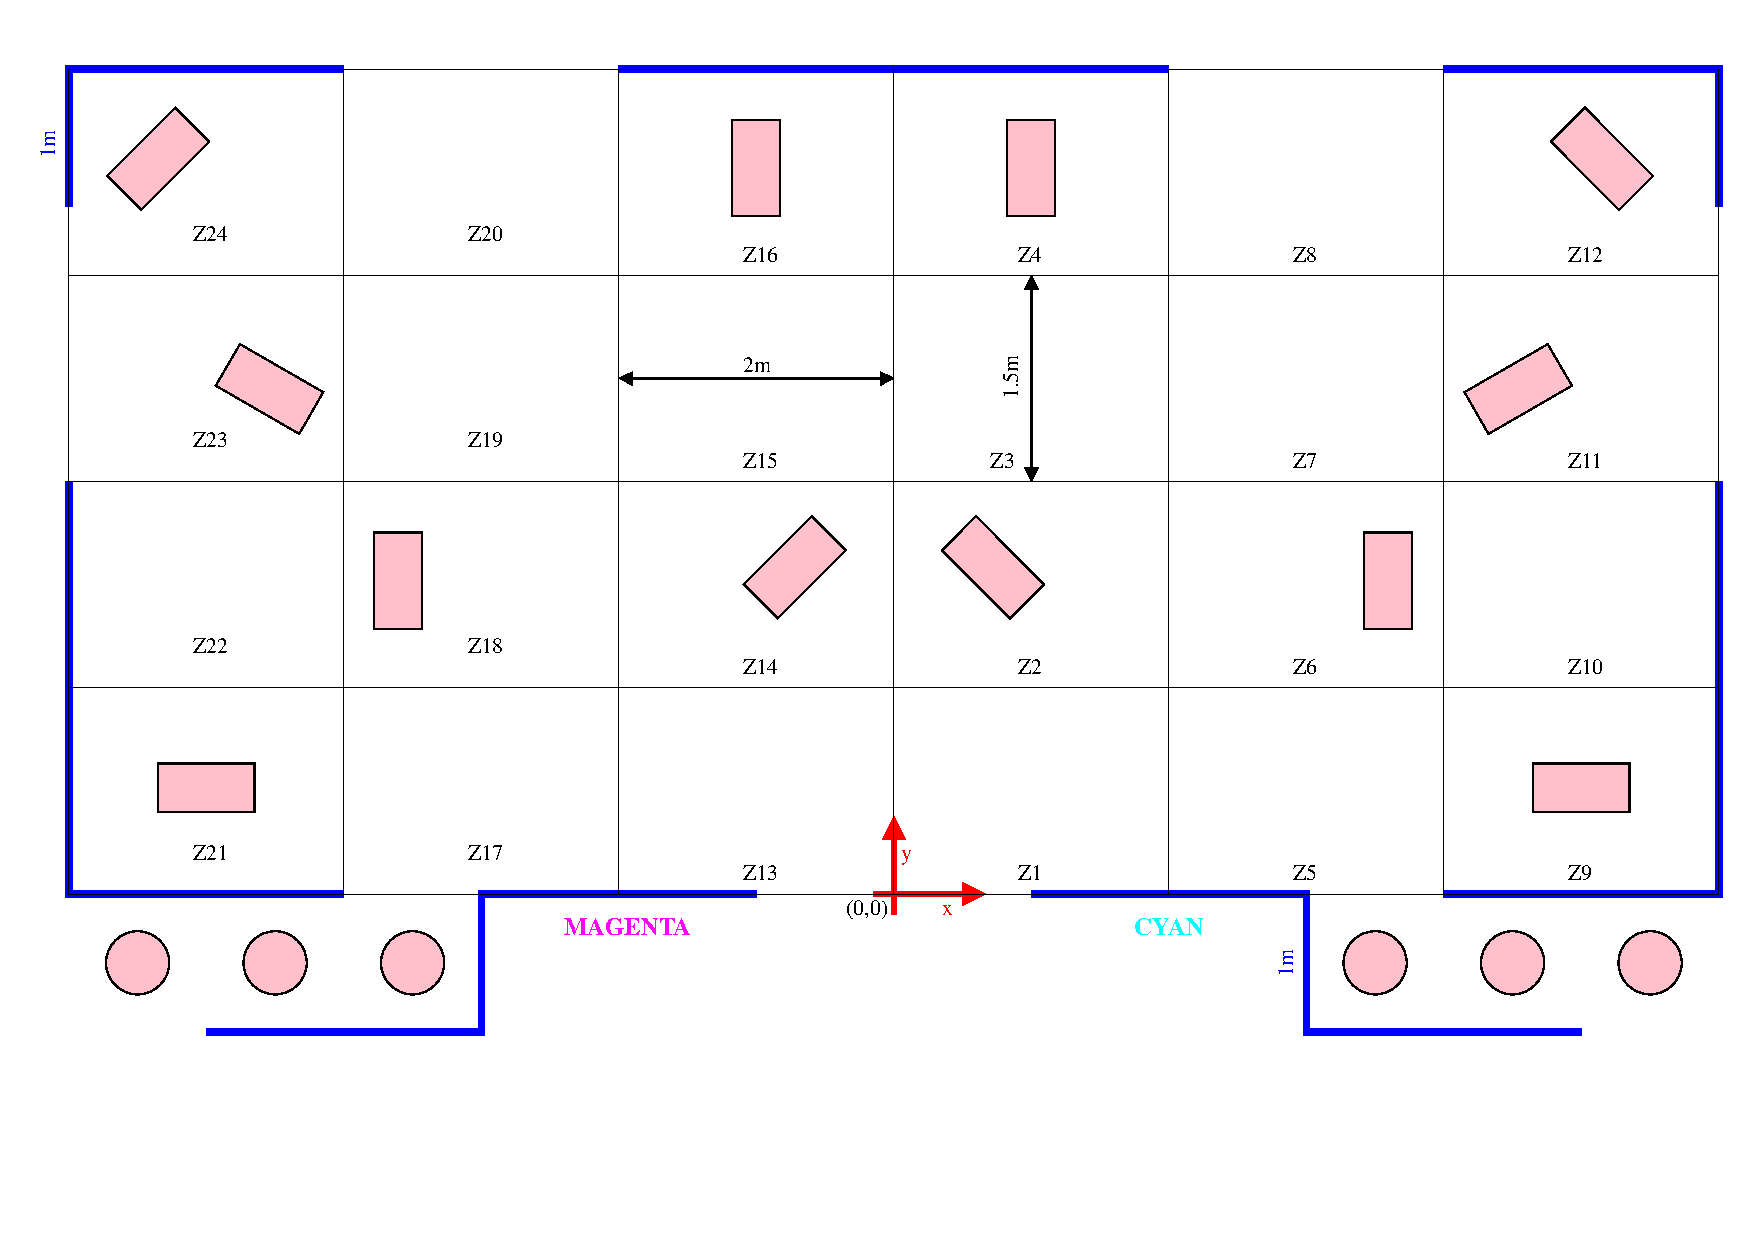
\includegraphics[angle=-90 , trim = 50 50 10 0, scale=0.85]{field.pdf}
  \caption{Competition Area}
\end{figure}

\subsection{Machines}
\label{sec:machines}
Machines are based on the Modular Production System (MPS)\footnote{For
  more information see
  \url{http://www.robocup-logistics.org/links/festo-mps}.} by Festo
Didactic Gmbh \& Co. KG. The MPS provides a number of stations which
make up the machines used in the competition. The stations have a
rectangular base shape of \SI{0,35 x 0,7}{\metre} with a height of
about \SI{1}{\metre} depending on machine type. Conveyor The machine
have individual application modules that provide different
functionality.

All machines share the same basic layout: a trolley, conveyor belt,
and signal unit. The markers are mounted at the same position on both
wide sides of the trolley. It is movable by four wheels with
\SI{0.1}{\metre} clearance. Both narrow sides of the trolley are
closed by plexiglas and have a handle. All physical interfaces
(conveyor belt input and output, shelves and set up slides for ring
stations are accessible at \SI{89.8}{\centi\metre} height. Working
space between guiding lanes is \SI{4.5}{\centi\metre}. Setup lanes and
shelves feature approximately the same space for handling and
adjusting. If observed from the output side of machines (where the
signal unit is placed) the conveyor space opens up at half of the
aluminum profile
% No clue what that means
%(visible by a break in the black plastic below),
thus starting at \SI{0,35}{\metre}. Based on these shared properties,
there are four kinds of machines:

\begin{description}
\item[Base Station (BS)] acts as dispenser of base elements
  (\reffig{fig:BS}, cf.~\refsec{sec:production-portfolio}). The
  application modules are three magazines of base elements. There is a
  single BS per team.

\item[Cap Station (CS)] mounts a cap as the final step in production
  on an intermediate product (\reffig{fig:CS}). The application module
  is a vacuum pick \& place module. A base element with a cap must be
  taken to the machine and is then unmounted and buffered in the
  machine. The cap is then mounted on the next intermediate product
  taken to the machine. There are two CS per team.

\item[Ring Station (RS)] mounts one colored ring out of two available
  colors on an intermediate product (\reffig{fig:RS}). Each RS has two
  vacuum pick \& place units as application modules with separate
  unique colors which are determined new for each game. There is an
  additionally pre-fill slide which is used for some colors (specified
  anew for each game) to add base elements. There are two RS per team.

\item[Delivery Station (DS)] Accepts completed products. The stations
  contains three conveyor belts (\reffig{fig:DS}). The robot has to
  choose the proper one for a specific orer. The delivered products
  are verified by either the referees or an automated external vision
  system. There is one DS per team.
\end{description}

\begin{figure}
  \centering
  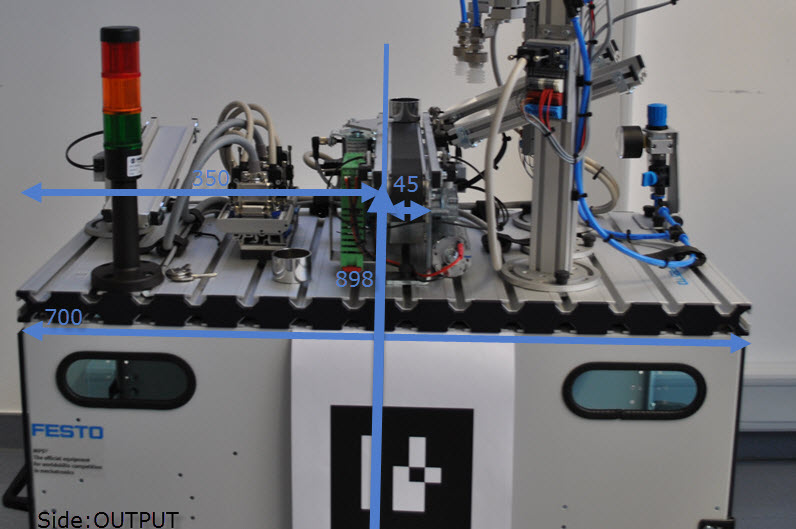
\includegraphics[height=7cm]{MPS2015/MPS_Layout.jpg}

  \caption{General Machine Layout}
  \label{fig:MPS-Layout}
\end{figure}
\begin{figure}
\centering
\subfigure[Base Station Portrait]{%
  \label{fig:BS_portrait}%
  \begin{minipage}[b]{0.3\linewidth}
    \centering
    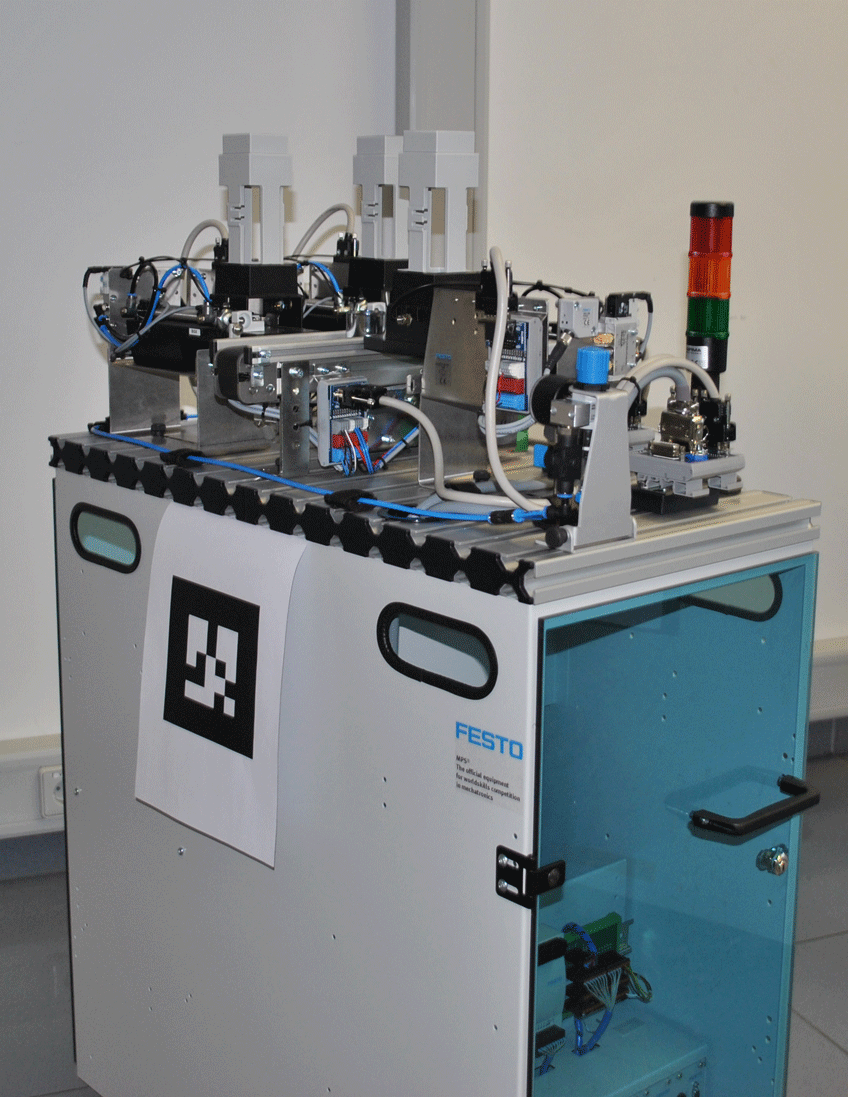
\includegraphics[height=6cm]{MPS2015/BS_portrait.png}
  \end{minipage}
} 
\quad
\subfigure[Base Station Output side]{%
  \label{fig:BS_Output}%
  \begin{minipage}[b]{0.55\linewidth}
    \centering
    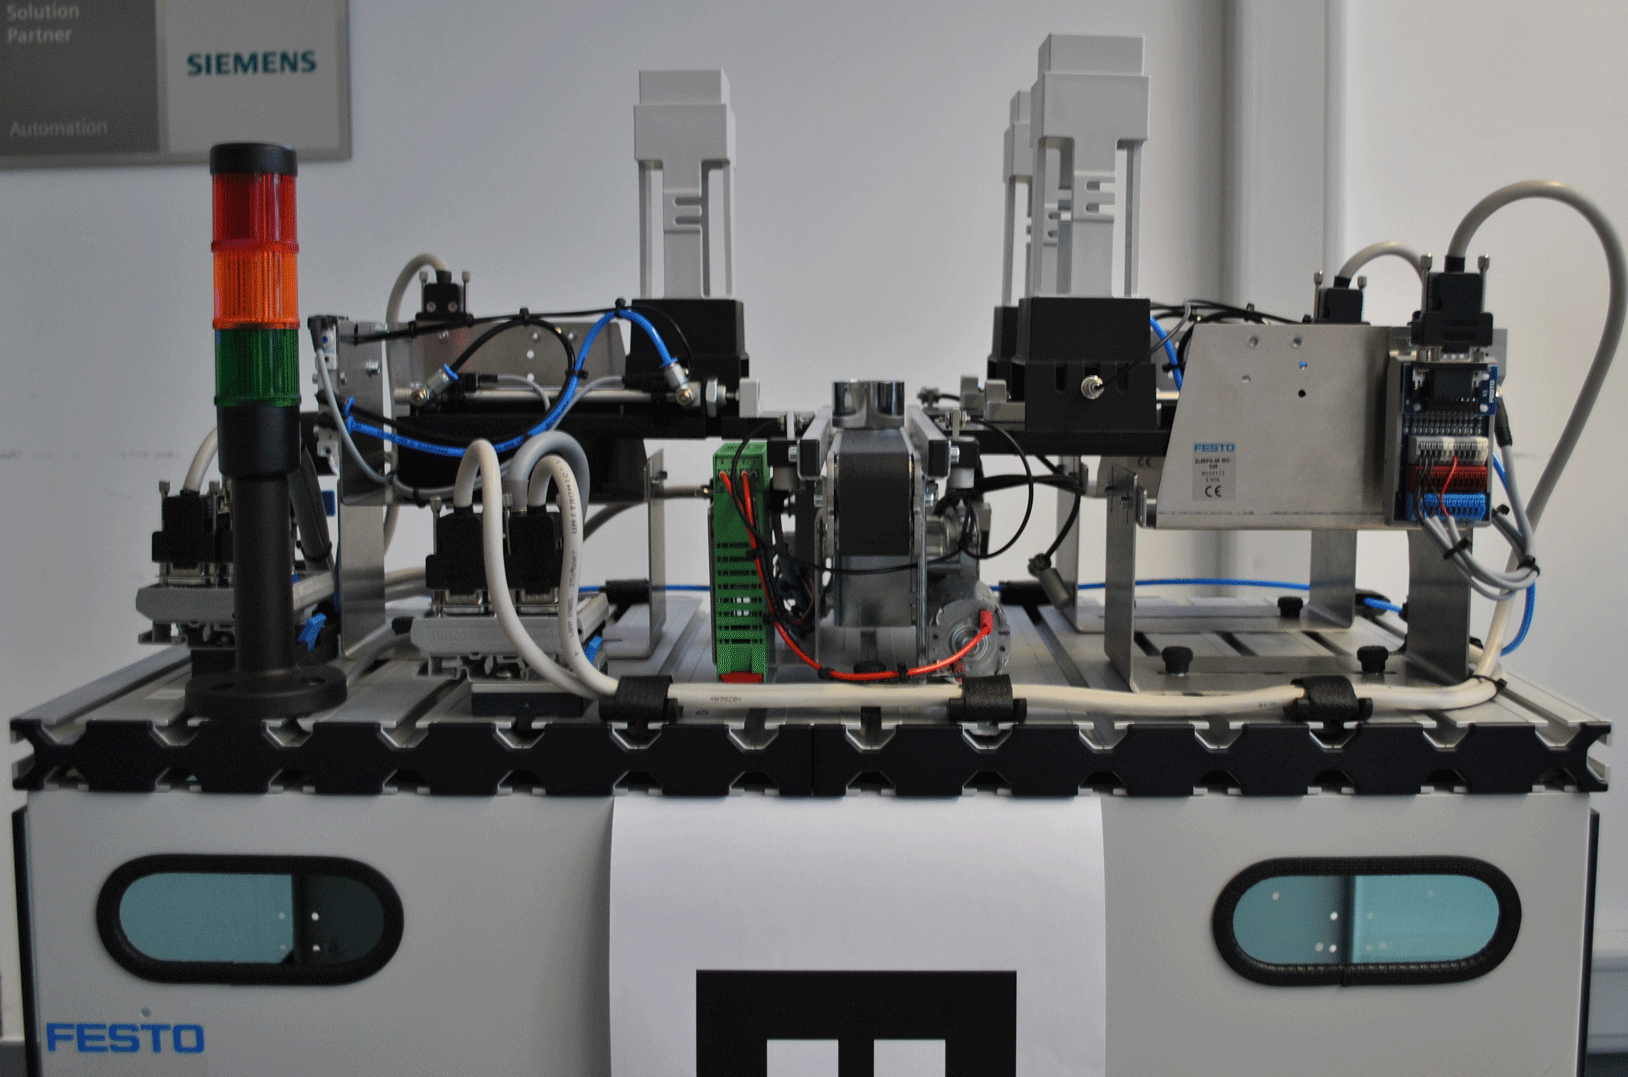
\includegraphics[height=6cm]{MPS2015/BS_Output.png}
  \end{minipage}
}
\vspace{-1ex}
\caption{Base Station}
\label{fig:BS}
\end{figure}
\begin{figure}
\centering
\subfigure[Cap Station Portrait]{%
  \label{fig:CS_portrait}%
  \begin{minipage}[b]{0.3\linewidth}
    \centering
    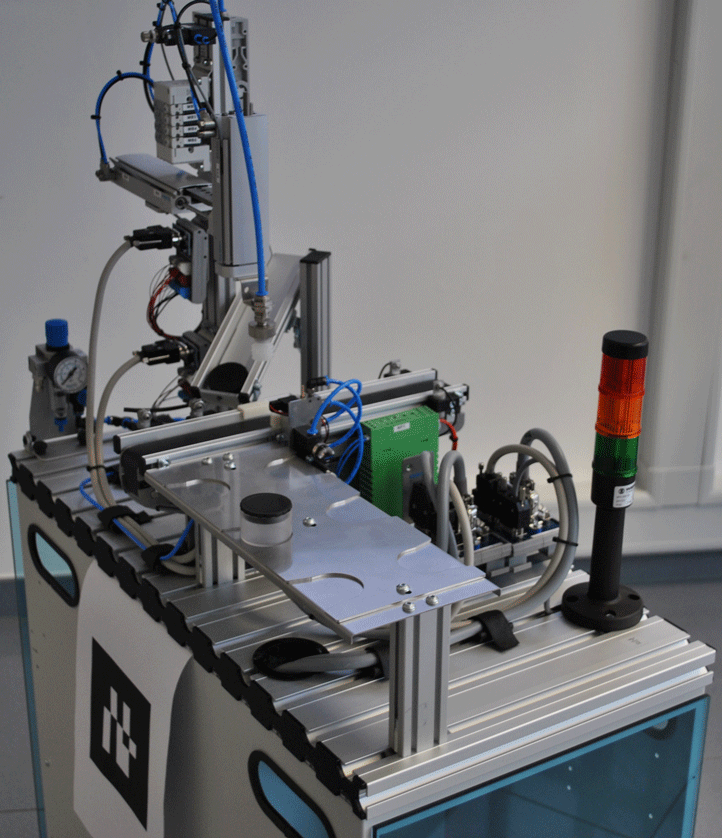
\includegraphics[height=6cm]{MPS2015/CS_portrait.png}
  \end{minipage}
} 
\quad
\subfigure[Cap Station Output side]{%
  \label{fig:BS_Output}%
  \begin{minipage}[b]{0.55\linewidth}
    \centering
    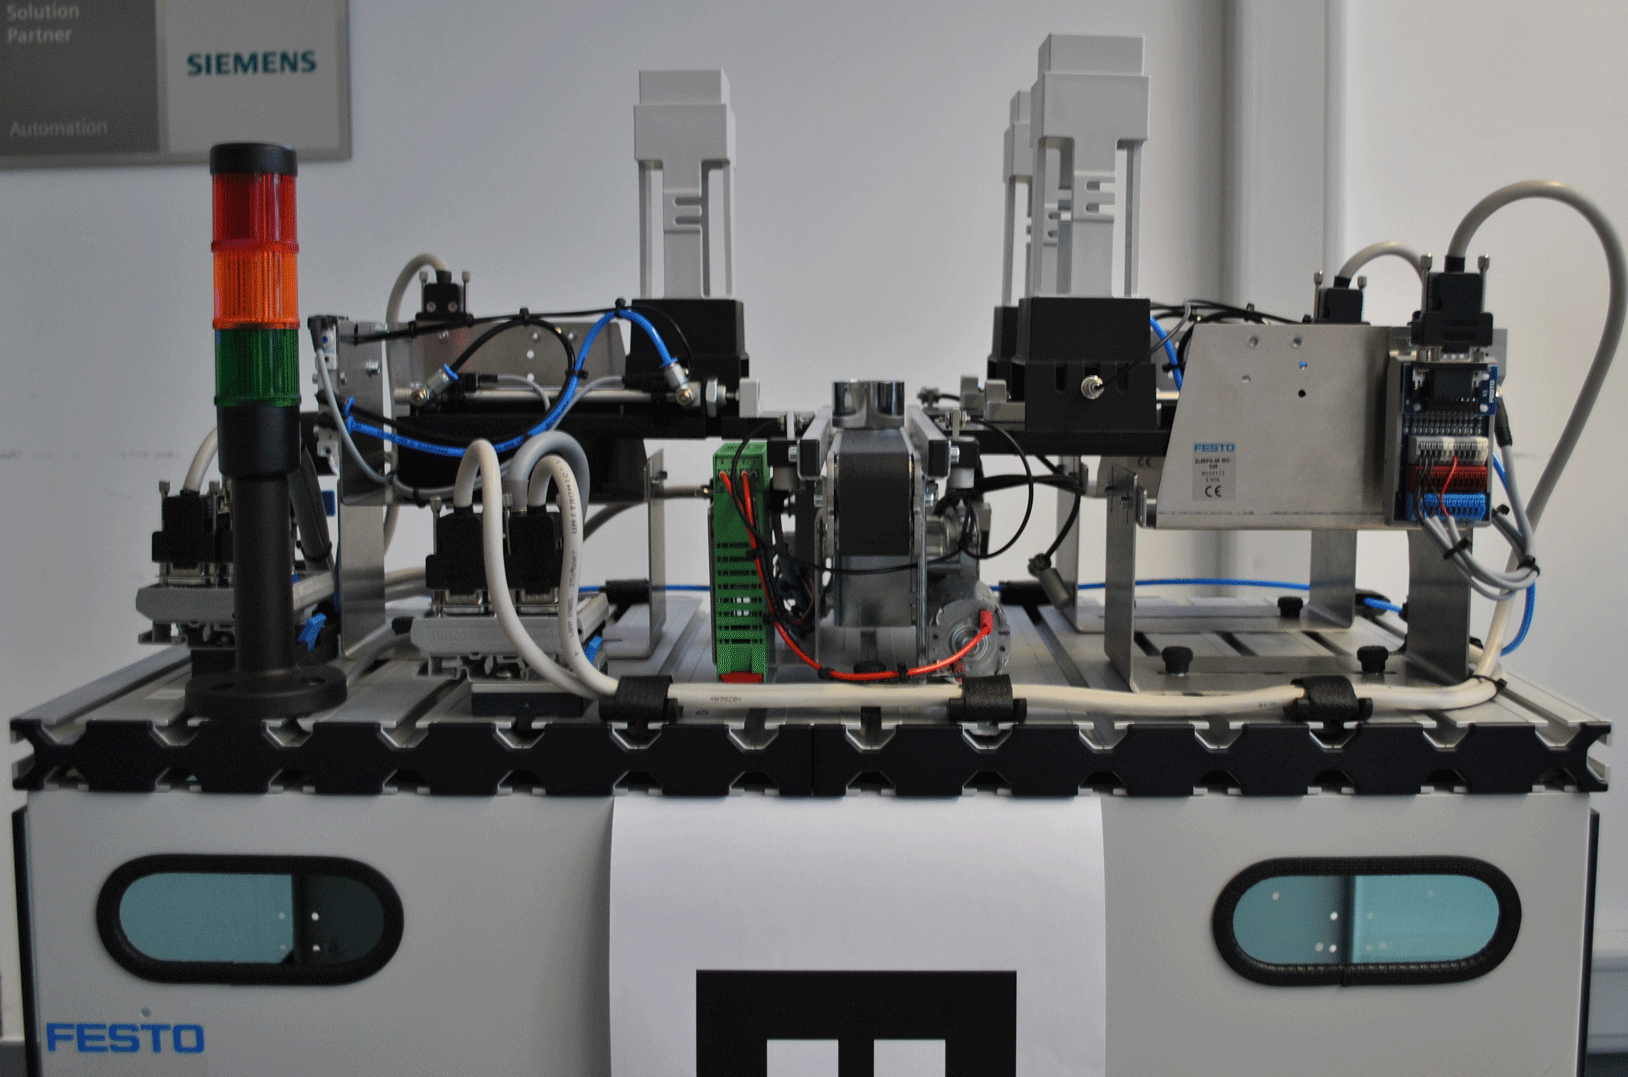
\includegraphics[height=6cm]{MPS2015/BS_Output.png}
  \end{minipage}
}
\vspace{-1ex}
\caption{Cap Station}
\label{fig:CS}
\end{figure}

\begin{table}[bp]
  \centering
  \begin{tabular}{|l|c|c|c|c|l|}
    \hline
    && \multicolumn{2}{c|}{Input} & \multicolumn{2}{c|}{Output}\\\hline
    &Machine & Tag ID & Tag & Tag ID & Tag\\\hline
    &&&&&\\[-2ex]
    \multirow{6}{*}{\rotatebox{90}{Cyan}}&
    CS 1&1&\parbox[c]{1.5cm}{
\includegraphics[width=1.2cm]{markers/figure_1}}&2&\parbox[c]{1.5cm}{
\includegraphics[width=1.2cm]{markers/figure_2}}\\[2.5ex]
    &CS 2&17&\parbox[c]{1.5cm}{
\includegraphics[width=1.2cm]{markers/figure_17}}&18&\parbox[c]{1.5cm}{
\includegraphics[width=1.2cm]{markers/figure_18}}\\[2.5ex]
    &RS 1&33&\parbox[c]{1.5cm}{
\includegraphics[width=1.2cm]{markers/figure_33}}&34&\parbox[c]{1.5cm}{
\includegraphics[width=1.2cm]{markers/figure_34}}\\[2.5ex]
    &RS 2&177&\parbox[c]{1.5cm}{
\includegraphics[width=1.2cm]{markers/figure_177}}&178&\parbox[c]{1.5cm}{
\includegraphics[width=1.2cm]{markers/figure_178}}\\[2.5ex]
    &BS&65&\parbox[c]{1.5cm}{
\includegraphics[width=1.2cm]{markers/figure_65}}&66&\parbox[c]{1.5cm}{
\includegraphics[width=1.2cm]{markers/figure_66}}\\[2.5ex]
    &DS&81&\parbox[c]{1.5cm}{
\includegraphics[width=1.2cm]{markers/figure_81}}&82&\parbox[c]{1.5cm}{
\includegraphics[width=1.2cm]{markers/figure_82}}\\[2.5ex]\hline

    &&&&&\\[-2ex]
    \multirow{6}{*}{\rotatebox{90}{Magenta}}&CS 1&97&\parbox[c]{1.5cm}{
\includegraphics[width=1.2cm]{markers/figure_97}}&98&\parbox[c]{1.5cm}{
\includegraphics[width=1.2cm]{markers/figure_98}}\\[2.5ex]
    &CS 2&113&\parbox[c]{1.5cm}{
\includegraphics[width=1.2cm]{markers/figure_113}}&114&\parbox[c]{1.5cm}{
\includegraphics[width=1.2cm]{markers/figure_114}}\\[2.5ex]
    &RS 1&129&\parbox[c]{1.5cm}{
\includegraphics[width=1.2cm]{markers/figure_129}}&130&\parbox[c]{1.5cm}{
\includegraphics[width=1.2cm]{markers/figure_130}}\\[2.5ex]
    &RS 2&145&\parbox[c]{1.5cm}{
\includegraphics[width=1.2cm]{markers/figure_145}}&146&\parbox[c]{1.5cm}{
\includegraphics[width=1.2cm]{markers/figure_146}}\\[2.5ex]
    &BS&161&\parbox[c]{1.5cm}{
\includegraphics[width=1.2cm]{markers/figure_161}}&162&\parbox[c]{1.5cm}{
\includegraphics[width=1.2cm]{markers/figure_162}}\\[2.5ex]
    &DS&49&\parbox[c]{1.5cm}{
\includegraphics[width=1.2cm]{markers/figure_49}}&50&\parbox[c]{1.5cm}{
\includegraphics[width=1.2cm]{markers/figure_50}}\\[2.5ex]\hline
  \end{tabular}
  \caption{Machine tags are ALVAR tags with the given IDs.}
  \label{tab:machine-tags}  
\end{table}
\begin{figure}[h]
\centering
\subfigure[Ring Station Portrait]{%
  \label{fig:RS_portrait}%
  \begin{minipage}[b]{0.3\linewidth}
    \centering
    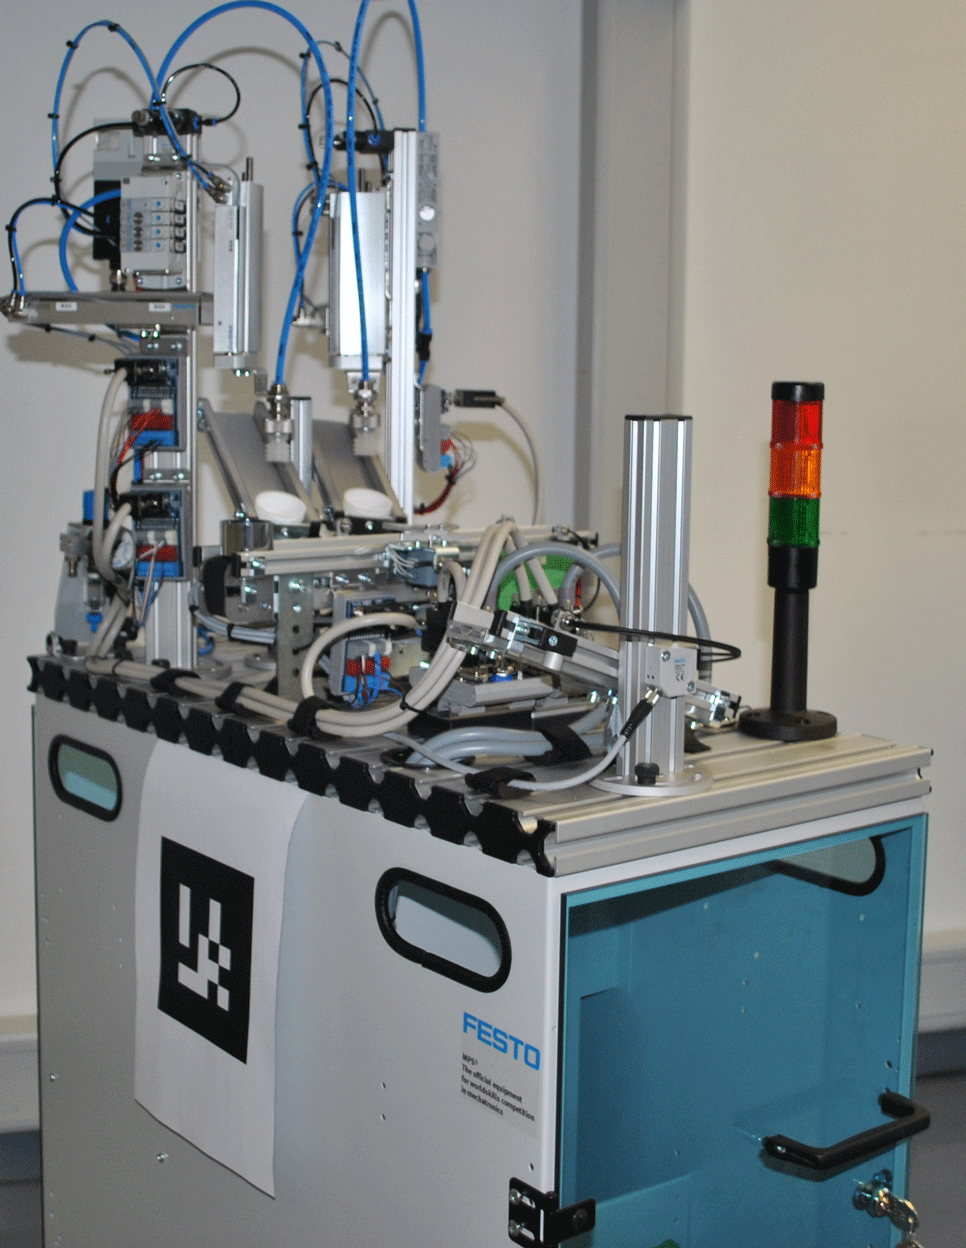
\includegraphics[height=6cm]{MPS2015/RS_portrait.png}
  \end{minipage}
} 
\quad
\subfigure[Ring Station Output side]{%
  \label{fig:BS_Output}%
  \begin{minipage}[b]{0.3\linewidth}
    \centering
    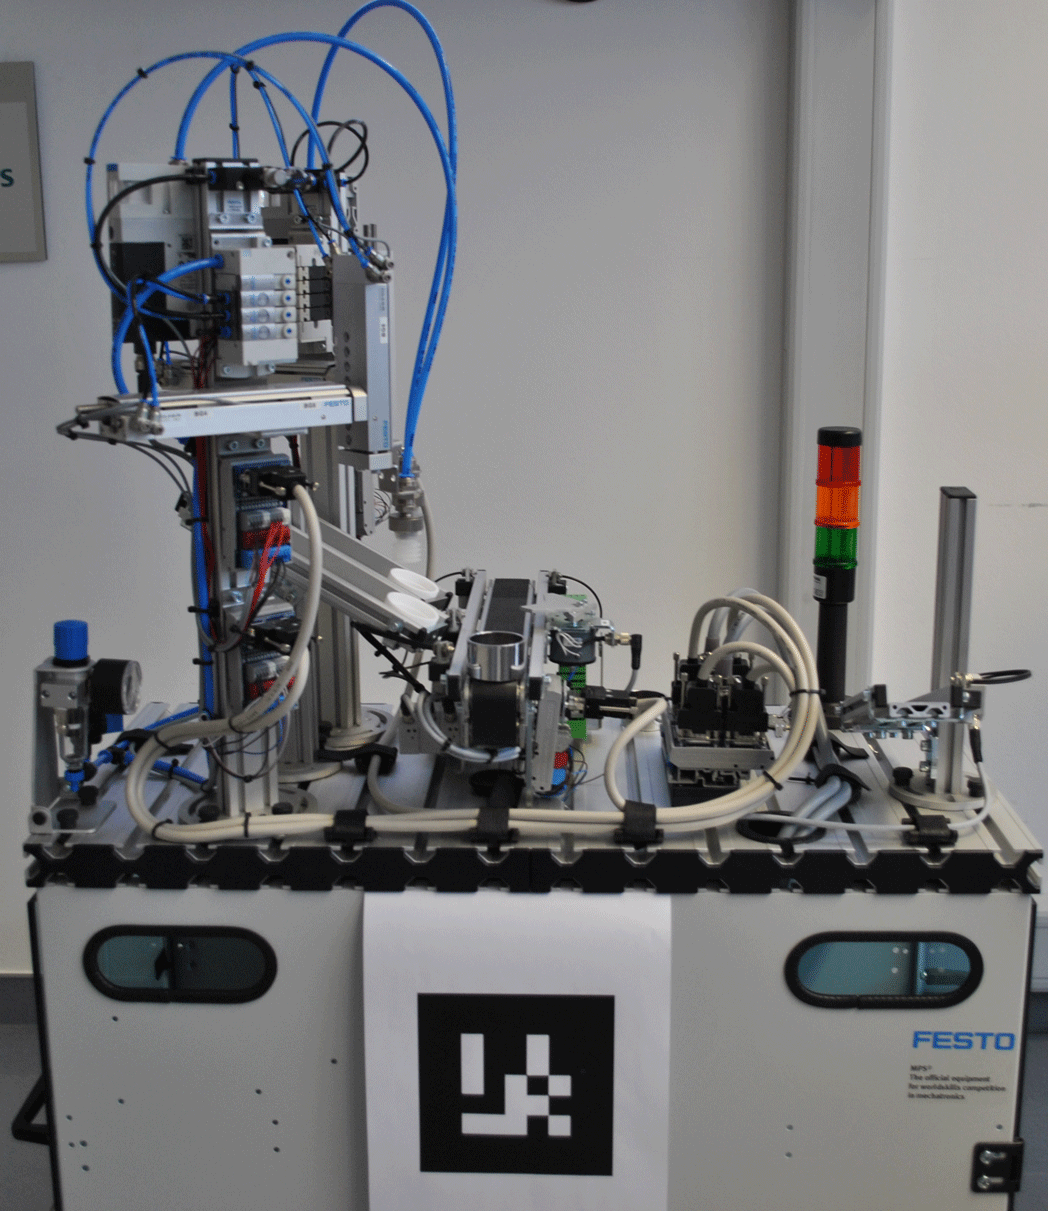
\includegraphics[height=6cm]{MPS2015/RS_Output.png}
  \end{minipage}
}
\vspace{-1ex}
\caption{Ring Station}
\label{fig:RS}
\end{figure}
\begin{figure}
\centering
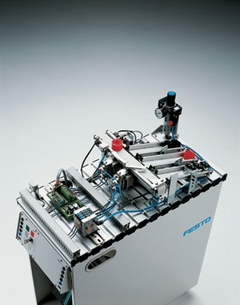
\includegraphics[height=6cm]{MPS2015/DS_portrait.jpg}
\caption{Delivery Station Portrait}
\label{fig:DS}
\end{figure}

\noindent
Machines of type CS and RS are called production machines as they
perform refinement steps on a product during the production phase.

\subsubsection{Machine Swapping}
\label{sec:machine-swapping}
Each team has a primary half
(cf. \refsec{sec:competition-area}). However, some machines will be
swapped, that is, some machines will not be located in the primary
half.

For each game, a CS and a RS of each team will be chosen randomly and
assigned to the one on the non-primary half -- that is two machines in
total per team. The CS and RS will be swapped with the symmetrically
positioned machine of the same type of the other team (machine types
remain unchanged).

\begin{table}[bp]
\centering
	\mytable{  \begin{tabularx}{\linewidth}{l|l|X}
    Type & Distribution & (Final) processing time[s]\\\hline
    Base Station (BS) & 1 per team & minimum physical time\\
    Cap Station (CS) & 2 per team & $t_2 = 15 \mbox{ to } 25~\mathrm{sec}$\\
    Ring Station (RS) & 2 per team &$t_3 = 40 \mbox{ to } 60~\mathrm{sec}$\\
    Delivery Station (DS) & 1 per team &$t_5 =20\mbox{ to } 40~\mathrm{sec}$
  \end{tabularx}}
  \caption{Production Machines - Type, Distribution and processing times}
  \label{tab:production-machines-function}  
\end{table}

\subsubsection{Production Machines -- During Exploration Phase}
\label{sec:production-machines-exp}
During the exploration phase the robots of each team can explore their
unknown factory environment by identifying where the different MPS are
located and what light signal pattern is shown.

The Referee Box assigns each machine to a team and a zone
(\reffig{fig:competition-area}) at the start of the exploration phase,
but the exact position and alignment within these and if this zone
contains an MPS at all will not be communicated. Each MPS is assigned
an individual light signal randomly. The light signal consists of a
steady light pattern, i.e. no flashing lights, resulting in seven
possible light states with at least one LED switched on. For details
how to perform the exploration phase
cf.~\refsec{sec:exploration-phase}.

After a successful report, the respective MPS will perform a dry run,
indicating visually for spectators that the MPS was indeed explored
successfully.\footnote{This feature is optional and may be left out.}

\begin{table}[tp]
  \centering
  \mytable{\begin{tabularx}{\linewidth}{p{0.36\linewidth}|X}
      \multicolumn{1}{l}{Optical Feedback} & \multicolumn{1}{l}{Operating mode} \\ \hline 
      All LEDs turned off & The machine is physically offline, caused by a real error, which should not happen during the competition. \\
      Red LED turned on & The machine is out of order. \\
      Red LED flashing (at 2 Hz)  & Machine signals that it ran out of stock on any required item. \\
      Green LED turned on & The machine is idle and ready.\\
      Green LED flashing & The machine has accepted the setup command
      (flashes for up to 3 seconds).\\
      Yellow LED turned on & The machine is currently busy.\\
      Red and yellow LED flashing (2 Hz) & A product was fed without
      proper setup of the machine \\%\hline
%%keep Red any Yellow one?
	\end{tabularx}}
  \caption{Production Machines - Optical Feedback during production phase}
  \label{tab:production-machines-feedback}
\end{table}

\vspace*{-2mm}
\subsubsection{Production Machines -- During Production Phase}
\label{sec:production-machines-production}
In the production phase production machine perform refinement steps on
a product such as mounting an additional ring or a cap. Machines
operate in a transaction style. That is, before using a machine it
must be setup for a specific mode. Then the input products can be fed
into the machine and the refinement step commences. Eventually, after
the production period is completed, the resulting product is delivered
on the output lane.

A light signal mounted near the output lane
(cf. \refsec{sec:machines}) to indicate the state of the machine. In
the default operating mode, the green light is turned on. This signals
that the machine is ready for setup or input. When setup is performed,
the green light will flash the green LED for up to 3 seconds (it
immediately switches to a new state, e.g. if a product is fed into the
machine before the three seconds are finished). When a product is fed
to the input, several light states indicate the processing
condition. If the machine accepts the input and starts processing the
green and yellow LEDs will be turned on steadily for as long as the
processing is performed. Once processing completes, the machine
switches back to a steady green LED only. If a product is fed for
which additional bases were required but which have not been
delivered, the machine will flash the red and yellow LED and will be
out of order (cf. \refsec{sec:broken-machine}). If an additional base
(cf.~\refsec{sec:production-phase}) is added to a machine the light
signal will change to steady orange. The light signals are summarized
in \reftab{tab:production-machines-feedback}.

In the production phase, machines must be setup before they can be
used. This applies to all machine types BS, DS, CS, and RS. If the
machine is not properly setup before used, it will go to a temporary
out-of-order state (cf.~\refsec{sec:broken-machine}).

The following describes the communication and reactions of the
machines during the production phase. For the actual messages we refer
to the integrator's manual~\cite{RefBoxIntManual}.

\begin{description}
\item[BS] The BS setup message denotes the color of the base element
  that should be dispensed. After receiving the message, the refbox
  will instruct the MPS to immediately provide a base of the desired
  color.
\item[DS] The DS setup message denotes the slide the product should be
  delivered to. The DS will consume any puck provided, but points can
  only be scored if the DS was properly setup.
\item[CS] The CS setup message initiates retrieval of a cap. The next
  base must be one with a mounted cap from the shelf. The cap is taken
  off the base and buffered. Afterwards the now cap-less base must be
  removed. The next intermediate product which is fed into the machine
  receives the buffered cap.
\item[RS] The RS setup message must state which of the two colors to
  prepare and retrieve. If the desired color requires additional bases
  (cf.~\refsec{sec:production-complexities}), the machine expects to
  receive them first. Once the required number of additional bases has
  been received, the intermediate product can be fed into the
  machine. It receives a ring of the desired color and moves the
  processed product to the output.
\end{description}

\noindent
The setup and use of a machine follows a transaction style. Once the
machine has been setup, the full cycle can be completed (committed).
But if a robot desires, it can cancel the production on the machine,
unless the intermediate product has already been fed into the
machine. Cancelling will invalidate any additional bases that have
been taken to the machine. There may be only one transaction running
at a time. If a second setup is performed without cancelling the
first, or if more bases are fed than required for the current
transaction, the machine will be temporarily broken
(cf.~\refsec{sec:broken-machine}).

\subsubsection{Recycling Machines}
Once a Cap Station (CS) has been supplied with set up material, the
empty base unit can be used to setup a Ring Station (RS) or be
recycled right away. It will not be possible to use the empty base
unit for further production.


\subsubsection{Delivery Station} 
\label{sec:delivery-station}
Once an order is completed, the product is has to be shipped to
Delivery Station (DS). After the physical interface, the Robot has to
command which of the three lanes is to be used to store the
product(which truck to load it on). More than one lane can be correct,
depending on the relevant order.

\subsection{Products}
\label{sec:products}
\todo[inline]{Fill in details about products.}
The rings come in the colors blue, green, yellow, and orange.

%%%%%%%%%%%%%%%%%%%%%%%%%%%%%%%%%%%%%%%%%%%%%%%%%%%%%%%%%%%%%%%%%%%%%%%%%%%%%
%%%

\section{Referees}
Referees manage the overall game, make sure that the rules of the game
are followed, and instruct and monitor the referee box.

\subsection{Referee Delegation}
Each participating team of the tournament must provide at least two
team members which act as referees. These referees must be announced
at the beginning of the tournament and are fixed throughout the whole
competition (unless the participant drops out of the tournament,
e.g. because of illness). The referees must meet the following
criteria. They must

\begin{itemize}
\item be available for each game that they are assigned to and appear
  5 minutes prior to the game start time (schedule to be announced by
  Organizing Committee at beginning of tournament)
\item have good knowledge of the rulebook and the applied rules
\item participate in the referee briefings (organized by Organization
  and Technical Committees)
\item be able to lead a game and communicate with the teams in
  English.
\end{itemize}

\subsection{Tasks and Responsibilities}
Each game requires 3 referees. One referee will run and oversee the
referee box. Two field referees observe the field, announce rule
violations, and communicate with the teams and refbox referee. Each
field referee is assigned to a particular field half. The referee
named first on the schedule is the head referee and is responsible for the 
team cyan and their corresponding field half. The head referee has
the upper hand when there is a referee disagreement and then announces
the final decision. The second listed referee assumes the liability of the 
team magenta.

The refbox referee has to operate the control machine during the game,
observe its status to ensure the correctness of the digital
representation and automatic scoring, announce critical situations to
the field referees, and start and stop the game on request of the
field referees. The refbox referee must also enter robot restarts and
observe the time remaining to bring back a robot, or announce if a
robot may no longer participate in the game (second restart).

The field referees observe the game from the side of the field or from
any position on the field (e.g., to better understand the game
situation). They shall avoid robots spatially on the field, but
ultimately robots are expected to avoid collision with human
referees. Field referees are also responsible for removing fallen products
from the playing-ground. Field referees are responsible for making the decision
whether a team may take out a robot for maintenance. And they observe
the correct refill procedure of their fieldhalf/team.

Each referee may call a pause of the game at any time, e.g. if robots
must be penalized or disentangled after a collision. Referees may
explicitly pause the game to convene and discuss an unclear situation
as to avoid hasty decisions. Such pauses shall be short-lived as to
follow the competition schedule.

\subsection{Liability Waiver}
Referees cannot be held liable for:
\begin{itemize}
\item any kind of injury suffered by a player, official or spectator
\item any damage to property of any kind
\item any other loss suffered by any individual, club, company,
  association or other body, which is due or which may be due to any
  decision, which he may take under the terms of the rules of the game
  or in respect of the normal procedures required to hold, play and
  control a match.
\end{itemize}

\subsection{Complaint Procedure}
Rule issues are not to be discussed during a game. Referee decisions
are binding for the game. A team may protest and challenge a game by
executing the following complaint procedure. The procedure is also
automatically invoked if a referee decides to abort a game for any
reason (e.g. field damage, lighting failures, burning robots).

To initiate the complaint procedure, the team leader of the
challenging team is to contact a member of the Technical Committee
within 10 minutes after the respective game has ended. The member of
the Technical Committee then invokes a team leader conference in
cooperation with the Organizing Committee. In this conference, the
following parties participate: the referees of the game in question,
not less than half of all registered team leaders, and the Technical
Committee (counseling). The situation shall be resolved by unanimous
consent or by vote of the team leaders (majority of team leaders
participating in the conference is sufficient).

All teams are reminded that while this is a competition, the league is
also about \emph{cooperative} research and evaluation and complaints
should be handled in a fair and forthcoming way.

\section{Game Play}
A match is defined by two contesting teams competing within the same
identical competition area. Each team consists of a maximum of 3
robots. Each match consists of 5 minutes of setup time, a maximum of 4
minute exploration phase, and a 15 minute production phase.
The three phases of the game are detailed below.

\subsection{Environment Setup}
\label{sec:env-setup}
The physical distribution and alignment of the production machines is
dynamic. The field will be organized as described in
\refsec{sec:competition-area}. The referee box will determine the
assignment of the machines to the zones at the beginning of a game
randomly. The machines will then be placed anywhere within their
assigned zone (similar on both sides of the field mirrored at the
field's Y-axis). The color for cap and ring stations will be
randomized prior to each match. The processing time of each production
step (i.e. per ring color and per cap mounting machine) will be
determined in the same way. The target delivery slide will be
randomized per order. During the setup phase
(cf.~\refsec{sec:setup-phase}) each team has the responsibility to
fill the input magazines on their base station. The elements may only
be touched by a robot or by designated persons after the game has
started.

% The robots can be set up within the factory area and have not been
% elevated into their autonomous state. Any necessary setup routine can
% be performed. This includes, but is not limited to, remote start-up of
% programs, localization procedures, or vision calibration.

\subsection{Interruptions and Robot Maintenance}
\label{sec:robot-maintenance}
During a match and while the robot is active on the field no manual
interference or manipulation of the robot in hardware, software,
configuration, instructions, or whatsoever, is allowed.  Teams may
visualize robot data on computers at the field, but existing keyboards
must be covered with a sheet of paper in order to assert a fair game
without manual interference.

% In the case of a misbehaving or broken robot, a team can ask the
% referee to take out a robot. Note, however, that one robot interfering
% with another is no conduct of misbehavior (unless damage is to be
% expected) and no reason to call out a robot. Similarly, to ask to take
% out a robot which is in a software deadlock situation of the own
% control software is not judged as a broken robot. The final decision
% whether a robot can be taken out or not remains with the field
% referee. The referee acts upon this motion at a time of his choosing,
% but as soon as possible.

Each team is allowed to maintain each robot once per game. The team
has to call upon the referee for \textit{robot maintenance}.  The
referee should judge the game situation carefully and should allow the
robot to be taken out for maintenance, if the calling team would have
any advantage in the current game situation from taking out the
robot. An advantage would be, for instance, to take out a robot, if
two robots of the same team are hindering each other. It is up to the
discretion of the referee when to allow the robot maintenance.

Because the new generation of Robotinos is relatively heavy and bulky,
up to two team members are allowed to remove a robot from the field.
Or the robots may be driven out manually by remote control using a
joystick, gamepad or similar. Human commands must be mapped directly
to motion commands, no autonmous driving is allowed. In both cases
(driving out and taking out) the robot must leave the field through
the closest opening in the wall unless this would interfere with the
game. In that case, the next closest exit maybe chosen (referee
decides). There will be a corridor (about \SI{1}{\metre}) around the
field where the can drive or be carried to the insertion area for
re-participation.

The repair time may take at most 120 seconds, starting from the moment
of driving or taking out the robot.  After a robot has been taken out
for the first time, the team can perform any repairs to the robot
and/or the robot's software. To return the robot into the game, the
team asks the referee to place back the robot onto the field. After
the referee accepts the motion, the team has 15 seconds quick setup
time, which is limited to basic instructions like initial localization
or software start-up. The robot may leave the insertion area onto the
field (autonomous driving). If the robot is not returned to the field
in time, it is disqualified from the ongoing game.

The referee can interrupt the game at any point in time, but should do
so rarely as not to interfere with the overall game flow (also
cf.~\refsec{sec:during-match}).

If a robot needs to be taken out for the second time, either on
request or as decided by the referee, it is disqualified from the
current game. It may no longer communicate with the still active
robots and must be taken out of the competition area.


\subsection{Game Start}
\label{sec:game-start}
%
All matches will start at the exact time scheduled by the organization
committee with the setup phase (cf.~\refsec{sec:setup-phase}). Once
the exploration phase starts, no more interference with the robot is
allowed. The robot must react to the referee box game state messages
to start the game play autonomously.

\subsection{Setup Phase}
\label{sec:setup-phase}
No team member is allowed to enter the competition area prior to or
during a match, except in cases of robot maintenance
(cf.~\refsec{sec:robot-maintenance}) or machine refill
(cf.~\refsec{sec:machine-refill}).  All robots which are to
participate in the game need to be in the insertion area during setup
(not in the game area where the machines are located). The referee box
will control the setup period and automatically switch to the
exploration phase after 5 minutes.

\subsection{Exploration Phase}
\label{sec:exploration-phase}
With the start of the exploration phase, the referee box announces the
mapping from zones to teams. As described in
\refsec{sec:production-machines-exp}, all MPS show a steady light
signal as randomly chosen by the referee box. The robots have 4
minutes to roam the environment and announce their 6 MPS for a
successful exploration to the referee box. Concretely, the referee box
expects a \emph{machine identified message} with a tuple consisting of
zone ID, machine ID (as encoded in the markers) and light
pattern. Please consult the referee box Integrator's
Manual~\cite{RefBoxIntManual} for a detailed definition of the message
types. Reports are only accepted for MPS of the respective team over
the private encrypted team channel. Only the first report for each MPS
is processed, all additional ones will be silently ignored. The
scoring is shown in \reftab{tab:scoring-exploration}. A minimum of
zero points will be accounted for the exploration phase. The
exploration phase ends either after the time has passed or immediately
after both teams have each reported their respective set of 6 MPS.

Moving or processing workpieces at an MPS is not allowed during the
exploration phase.

\subsection{Production Phase}
\label{sec:production-phase}
With the end of the exploration phase the production phase begins,
which lasts \num{15} minutes. The referee box publishes information
regarding products and machines. This includes machine zones and
contained colors of ring and cap stations, as well as the different
product variants that can be produced
(cf.~\refsec{sec:production-portfolio}). The refbox posts orders
(cf.~\refsec{sec:production-plan}) which then must be fulfilled by the
robot teams. Using production machines requires interaction through
communication with the refbox described in
\refsec{sec:production-machines-production}.

Starting with the play-offs phase of the tournament
(cf.~\refsec{sec:tournament-phases}) the game must be won by one of
the teams by a higher score. If after the regular game time there is a
draw, the game will automatically and without interruption be extended
by 5 more minutes. If after five minutes there is still no winner, the
team scoring the first points will win. If no points were scored a
coin toss decides.

\subsubsection{Production Portfolio}
\label{sec:production-portfolio}
\begin{figure}
  \ffigbox{%
    \centering
    
    \hfill
    \subfigure[$C_0$]{\label{fig:prod-compl-0}%
      
\includegraphics{prod2015/c0_black_gray}
    }
    \hfill
    \subfigure[$C_1$]{\label{fig:prod-compl-1}%
      
\includegraphics{prod2015/c1_red_blue_black}
    }
    \hfill
    \subfigure[$C_2$]{\label{fig:prod-compl-2}%
      
\includegraphics{prod2015/c2_silver_blue_green_black}
    }
    \hfill
    \subfigure[$C_3$]{\label{fig:prod-compl-3}%
      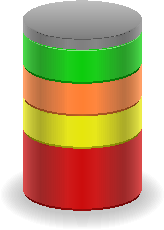
\includegraphics{prod2015/c3_red_yellow_orange_green_gray}
    }
    \hfill\,
    
}{%
  \caption{Products are composed of a base element and a cap with
    zero, one, two, or three intermediate rings representing the
    product complexity. The complexity level is stated as the number of
    required intermediate rings. The base element colors are red,
    black, and silver, the ring colors are blue, green, yellow, and
    orange, and the cap colors are either gray or black.}
  \label{fig:production-complexities}
}
\vspace{-1mm}
\end{figure}
The production portfolio is composed of three elements
(cf.~\refsec{sec:products} for specifications) specified below. The
machine handling is described in~\refsec{sec:machines}.

\begin{description}
\item[Base] The base is the lowermost element in each production. Only
  a base shall be grasped by a robot. Bases are dispensed by the base
  station (BS) and bases with mounted caps are available on the cap
  stations (CS). Bases are available in the colors red, black, and
  silver.
\item[Ring] Rings are mounted in intermediate production steps at ring
  stations (RS). A production features, zero, one, two, or three
  intermediate rings of distinct color
  (cf.~\refsec{sec:production-complexities}). The order of the rings
  matters. Each RS is responsible for two specific colors. Some colors
  require loading the RS with additional bases
  (cf.~\refsec{sec:production-plan}).
\item[Cap] Caps are the topmost element in each production. They are
  obtained by taking pre-assembled base-cap combinations available on
  the shelf to the cap station (CS). The CS unmounts the cap and loads
  it to its internal buffer. Then, the actual production element
  (consisting of a base and up to three rings) must be placed in the
  machine and the cap is mounted.
\end{description}

\subsubsection{Production, Color Complexities, and Additional Bases}
\label{sec:production-complexities}
The portfolio comprises many different product variants and is
categorized by the four available \emph{product complexity} levels
shown in \reffig{fig:production-complexities}. The lowest complexity
$C_0$ requires to load the CS with the proper cap color and then
processing a properly colored base at that machine. The highest
complexity $C_3$ requires a base with three mounted rings and a
cap. For a product, the colors of base, rings, and cap as well as the
order of the rings are of importance.

The product complexities do not account for \emph{additional bases}
that are required for some colors. We distinguish \emph{color
  complexities} as $CC_0$, $CC_1$, and $CC_2$ depending on whether
zero, one, or two additional bases are required for a color. The
referee box ensures that there will always be some orders for $C_1$
products where the ring color does not require additional bases,
i.e. with color complexity $CC_0$ -- but not necessarily all $C_1$
orders have this constraint.

\begin{figure}[h]
  \ffigbox{%
    \centering
    \begin{minipage}{0.75\linewidth}
      \subfigure[Production of complexity $C_0$ only mounting a cap on a
      BE as shown in \reffig{fig:prod-compl-0}.]{
        \label{fig:prod-chain-C0}%
        \begin{minipage}{1.0\linewidth}
          \centering
          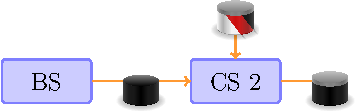
\includegraphics{prod2015/chain_c0}
        \end{minipage}
      }
      \subfigure[Production of complexity $C_1$ with a single intermediate
      ring according to \reffig{fig:prod-compl-1}.]{\label{fig:prod-chain-C1}%
        \begin{minipage}{1.0\linewidth}
          \centering
          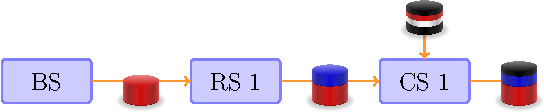
\includegraphics{prod2015/chain_c1}
        \end{minipage}
      }
    \end{minipage}
    \quad
    \subfigure[Legend]{
      \label{fig:prod-chain-legend}%
      \begin{minipage}{0.2\linewidth}
        \centering
        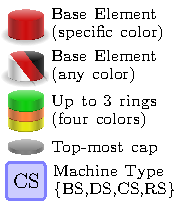
\includegraphics{prod2015/legend}
        \vspace{2mm}
      \end{minipage}
    }


    \subfigure[Complexity $C_2$ with two rings
    (cf. \reffig{fig:prod-compl-2}). RS 2 requires an additional base
    (of any color) for the green ring.]{\label{fig:prod-chain-C2}%
      \begin{minipage}{1.0\linewidth}
        \centering
        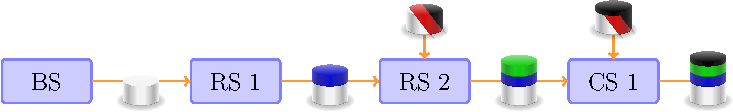
\includegraphics{prod2015/chain_c2}
      \end{minipage}
    }

    \subfigure[Production of the highest complexity $C_3$ with a three
    intermediate rings according to \reffig{fig:prod-compl-3}. Note
    that RS 2 requires two additional BE (of any color) for the orange
    ring and another one for the green
    ring.]{\label{fig:prod-chain-C3}%
      \begin{minipage}{1.0\linewidth}
        \centering
        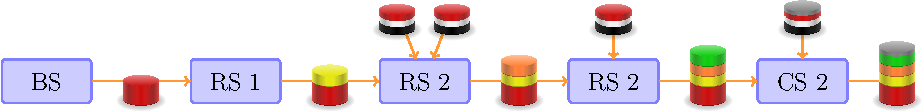
\includegraphics{prod2015/chain_c3}
      \end{minipage}
    }

}{%
  \caption{Production Chains of four example products
    (cf. \reffig{fig:production-complexities}). Blue boxes represent
    machines. RS 1 mounts yellow and blue, and RS 2 orange and green
    rings. Mounting an orange ring requires one additional BE (of any
    color). Similarly two additional BE are required for a yellow
    ring. Cap stations require a BE (of any color) with a cap of the
    matching required color.  \emph{Note that this is a particular
      example. The actual production chains and requirements for
      additionale BEs are determined randomly by the referee box for
      each game}.}
  \label{fig:production-chains}
}
\vspace{-1mm}
\end{figure}
\subsubsection{Production Plan}
\label{sec:production-plan}
The referee box will announce orders throughout the game in an
incremental fashion. Each order will consist of the product to
produce, the amount thereof, and a delivery time slot. An order
therefore specifies a production chain to be accomplished for
fulfillment. \reffig{fig:production-chains} shows some example
production chains of the four different complexities. The complexity
is specified by the number of required intermediate rings from $C_0$
(no ring) to $C_3$ (three intermediate rings). As specified in
\refsec{sec:production-complexities}, some specific steps require
additional bases to be added to the machine after setup
(cf.~\refsec{sec:production-machines-production}). This depends on the
specific color, it is randomized per game and announced by the refbox.

In each game, orders with a fixed delivery value of 160 points will be
placed\footnote{This number is currently a best guess as experience
  with the new production plan is not yet available. The number can be
  adjusted during the tournament by the Technical Committee, should
  this turn out to be necessary.}. These points only include the final
production step and delivery. The complexities of orders will be
similar for all games within a phase. But the actual production chains
are randomized. Each order will require one or more products of a
specified product type to be delivered. The product is specified in
terms of base color, rings (color and order), cap color, and possibly
delivery gate. The delivery time slot will have a randomized start
time. The duration will be randomized between 30 to 180 seconds. The
end time shall be within the game time. The duration shall be long
enough to cover at least the production time of the final machine in
the production chain and 30 seconds of travel time. The orders shall
be posted with a uniform distribution over the whole game time (but
there is not necessarily an open order for a particular product at a
specific time, or any order at all). The first order will be posted
within the first 120 seconds of the game (but not necessarily at the
beginning of the game). Orders for the products of complexity $C_2$ or
$C_3$ will not begin in the first 300 seconds. An order will be
announced before the delivery time slots starts. For $C_0$ and $C_1$
products the time ahead of the start of the time window is 10 to 60
seconds, for $C_2$ and $C_3$ orders the time is between 60 and 300
seconds. Two early orders will be posted that are announced at least
300 seconds ahead of time in the first third of the production phase.

In all tournament phases (cf.~\refsec{sec:tournament-phases}), the
teams playing on the field at the same time will get the same
production plans, but other games will have their own.

The multi-staged production processes can be repeated as long as
enough material can be provided to complete the cycle (also
cf.~\refsec{sec:machine-refill}). The different machine types are
specified in Section~\ref{sec:machines}.

\subsubsection{Machine Refill}
\label{sec:machine-refill}
The teams are responsible for refilling the machines (base elements,
rings, and caps). Each team has to designate one team-member as a
\textit{"replenisher"}.  This replenisher must be specified to the
corresponding "field half/team" referee before each game.  Only this
team member will be allowed to access the field area and only in case
of a recent refill procedure.  The replenisher must not obstruct other
robots and should interfere as little as possible.  The machines can
only be refilled when a magazine is empty and the machine indicates
this (flashing red light). In this case the field-operator may enter
the competition-area without asking the referee.

\subsection{Special Events during a Match}
\label{sec:during-match}
Any referee can interrupt the match at any time. After the referee box
is stopped, all robots have 3 seconds to stop all robot movement.
Robots that do not stop within the time limit will be treated in the
same way as misbehaving robots (cf.~\refsec{sec:robot-maintenance}).
The match time will be paused during the interruption.

\subsubsection{Scheduled Machine Downtime}
\label{sec:out-of-order}
The refbox will take down machines randomly out of the pool containing
the RS and CS. It will do so at random points of time and with the
same conditions for both teams, i.e., affecting the same machines for
both teams. There will be 2 to 4 of such triggered events during a
match. The machines affected will remain out of order for 30 to 60
seconds. Every machine can only be forced out of order once per
match. If a machine turns offline during processing or consumption of
mounted a pallet carrier, it will afterwards resume the process
(extending the overall processing time by the down time). The downtime
is indicated by a steady red light.

\subsubsection{Broken Machine Downtime}
\label{sec:broken-machine}
If a machine is improperly instructed or used, the machine will go
into a failure state. The machine cannot be used for 30 seconds and
until repaired. That is, if damage was inflicted on the machine or the
referee needs longer to repair the machine the game continues and the
machine will be offline for a longer time. Any production that was
running will be aborted and any product which was being processed is
no longer available and will be removed by the referee. Any additional
bases delivered to the machine will be void. The downtime is indicated
by a flashing red light.

\subsection{Task Fulfillment and Scoring}
Table \ref{tab:scoring} provides the itemized clearance of all task
related processes and their scoring. Note that all points related to a
product, including the points for finishing intermediate step like
mounting the last ring on higher complexity products, are awarded on
delivery only. Products, which are not delivered, do not score. That
includes half-finished products at the end of the game in particular.
Production points are also awarded for later deliveries, that is,
points for steps like mounting the cap are awarded in full for as long
as there was or is an order active for that specific product if there
are still items in the order remaining, i.e. not the full amount of
ordered products has been delivered.
\begin{table}
  \centering
  
    \subtable[Scoring scheme for the exploration phase]{%
      \label{tab:scoring-exploration}   

      \mytable{\begin{tabularx}{\linewidth}{p{7em}|X|p{4em}}
        \multicolumn{1}{l}{Reported} &\multicolumn{1}{l}{Exploration Phase} & \multicolumn{1}{l}{Points}\\\hline
    Correctly & Correctly determine a machine type of your team and
    report it successfully to the refbox &	+8\\
    Incorrectly & Wrongly reported machine type &  -6\\
    Round Total & A maximum of 48 points can be achieved by correctly
    reporting all 6 production machines. A minimum of 0 points is
    awarded. & 0 -- 48\\%\hline
  \end{tabularx} }}%

\bigskip%

  \subtable[Scoring scheme for the production phase]{
    \label{tab:scoring-production}   
    \mytable{
      \begin{tabularx}{\linewidth}{p{7em}|X|p{4em}}
        \multicolumn{1}{l}{Sub-task } &\multicolumn{1}{l}{Production
          Phase} & \multicolumn{1}{l}{Points}\\\hline
        Finish $CC_1$ step & Finish the work order for a color requiring one additional base & $+4$\\
        Finish $CC_2$ step  & Finish the work order for a color requiring two additional bases & $+8$ \\
        Finish $C_1$ pre-cap & Mount the last ring of a $C_1$ product & $+4$ \\
        Finish $C_2$ pre-cap & Mount the last ring of a $C_2$ product & $+8$ \\
        Finish $C_3$ pre-cap & Mount the last ring of a $C_3$ product & $+12$ \\
        Mount cap & Mount the cap on a product & $+2$ \\
        Delivery & Deliver one of the final product variants to the
        designated loading zone at the time specified in the order & $+20$\\
        Late Delivery & An order delivered within 10 seconds after an
        order is awarded a reduced score. For delivery time slot end
        $T_e$ and actual delivery time $T_d$ in seconds the reduced
        score is given by $20 - \lfloor T_d - T_e \rfloor * 2$.
        & up to $+20$\\
        Wrong delivery & Deliver one of the final product variants to
        the designated loading zone out of the requested time range or
        after all products requested in the period have already been
        delivered
        & $+1$\\
        False delivery & Deliver an intermediate product & $0$\\
        Just-in-time Production & The cap of a successfully delivered
        good has been mounted within the
        order time window& $+5$\\
        Recycle & Taking a consumed material from a machine that
        completed its work cycle to the recycling machine& $+5$\\
        Obstruction Penalty & Deliver a data carrier to a machine, which belongs to the opposing team. & $-2$ \\
      \end{tabularx}
    }
  }

	\bigskip

	\subtable[Scoring scheme for game commentary]{\mytable{\begin{tabularx}{\linewidth}{p{7em}|X|p{2.4em}} \multicolumn{1}{l}{Task} &\multicolumn{1}{l}{Game Commentary} & \multicolumn{1}{l}{Points}\\\hline
      Accepted Commentary & Commentate at least one half of the game continuously
      on microphone in English to the public. &  +10\\%\hline
  \end{tabularx} }}
  
  \caption{Scoring Schemes}
  \label{tab:scoring}   
\end{table}

\subsection{Obstruction Penalty}
\label{sec:obstruction-penalty}

As the Logistics League follows the idea of having both active teams 
compete alongside each other, instead of directly against each other, we 
punish intentional obstruction of the opposing team.

Especially, this applies to the input and output area in front of any MPS. 
All robots are allowed to enter this space, but robots must not obstruct 
opposing robots which intend to approach their MPS. Concretely, that robot 
must give way and release an approachable path to the MPS within a time window 
of 10 seconds. If a robot cannot follow this rule, a pushing foul will 
be called according to Section \ref{sec:pushing-rules}.

% old ?!
Furthermore, teams are penalized with -2 points for obstruction when delivering a
workpiece to a machine of the opposing team.  In this case, the
workpiece becomes junk and cannot be recycled or used afterwards. If the
robot leaves the machine space without the workpiece, the workpiece will be
removed by a field referee.

\subsection{Pushing Rules}
\label{sec:pushing-rules}

With multiple teams on the field at the same time, robots must
implement ways for collision avoidance. At the same time, they shall
not interfere with the goods of the other team. The case where a robot
of one team bumps into or moves a robot of another team we
call ``pushing''.

The following rules shall be obeyed by the robots and provide the
guidelines for referees to call for improper behavior of a robot due
to pushing.

\begin{enumerate}
\item Pushing occurs only between robots of different teams.
\item Robots must drive such that they try to avoid physical contact
  with robots from the opposing team. However, physical contact per se
  does not represent an offense.
\item All robots should be equipped with appropriate sensors to detect 
situations of physical contact with other robots (direct pushing situations).
\item If physical contact with other robots cannot be avoided, it must
  be soft, i.e. at slow speed and with as small physical impact as
  possible, in order to avoid damage to itself and other
  robots. Robots moving at high speed must significantly decelerate
  before a collision occurs with another robot.
\item If a destruction collision is immediate and the robots don't
  react, the referee should use the refbox to send a stop command to
  all robots. Every team has to react to the stop command by
  immediately stopping their robots.
\item Whenever a robot produces direct physical contact with another
  robot while moving, it must stop movement immediately in that
  direction (and choose a new direction for movement).
\item If pushing occurs between a moving and a standing robot, the
  moving robot causes the pushing situation and is responsible for
  resolving it. If it is not able to do so, a pushing foul will be
  called.
\item If pushing occurs between two moving robots, both robots are
  responsible for resolving the pushing situation. If one robot
  continues pushing by moving in its initial direction, while the
  other robot is recognizably reacting and trying to take another
  direction, the foul will be called on the pushing robot.
\item If two robots encounter physical contact and cannot resolve the
  situation because they get entangled, the referee may issue a
  pushing foul on both robots.
\item If, in the opinion of the referee, physical contact between two
  robots is not soft, or if one or both of the robots do not change
  direction after encountering physical contact, a pushing foul will
  be called.
\item When a pushing foul is detected the responsible team has to use
  up their restart for the stuck robot to start at the insertion zone
  again. The other team can decide within 10 seconds to restart their
  involved robot in the insertion zone without it counting as a
  penalty restart.
\item Moving a workpiece of the opposing team at their MPS is a pushing 
foul. The referee will move the workpiece back to its original position.
\item Intentional obstruction of the opposing team is a pushing foul, as 
described in Section \ref{sec:obstruction-penalty}.
\item If a robot is restarted or called to maintenance, loses his 
workpiece during collision avoidance or in case of a collision, the 
workpiece will not be replaced and is removed by the referee.
\item The league reserves its right to disqualify clearly malicious
  teams.
\end{enumerate}

\section{Tournament}
\label{sec:tournament}
The tournament is organized in a main competition and three technical
challenges. Teams can decide to participate in any of those.

\subsection{Tournament Phases}
\label{sec:tournament-phases}
There will be three stages in the main competition, a round-robin
phase for all participating teams, playoffs for the best four teams
from the round-robin phase, and the finals. The best two teams of the
playoffs play the grand finale to decide which team will become the
next Logistics League champion, whereas the other two teams compete in
the small final for the third place.

\paragraph{Round-Robin phase.~} 
The first stage is a group phase and will be played as a round-robin.
The teams will receive the true points they scored during the
competition. The points will be accumulated in this phase and the
teams will be ranked according to the accumulated points in descending
order.

\paragraph{Playoffs.~}
At the playoff stage, the scoring scheme will be different. As each
team in this phase directly competes with an opposing team, the team
that scores more points as the direct opponent, will be announced as
the winner and 3 points will be awarded to this team. A loss will be
awarded with 0 points. Additionally, if both teams are unable to score
any points during the match by delivering or producing goods, both
teams will receive 0 points. In case of a draw within the playoffs,
the game time will be extended by 5 minutes unless both teams scored
zero points. This will be announced by the refbox instead of a game
closed message.
%
If this extension leads to a draw too, the overall regular points of
the teams will determine the match winner. If the overall points are
equal too, a direct comparison between the teams in question will
decide. If this fails to resolve the situation, the teams will
approach a coin toss to determine the winner.

\paragraph{Finals.~}
The best two teams of the playoff phase will advance to the grand
finale, the remaining two teams will compete in the small finals for
the third place. The team that scores more points after the regular
game time wins. If there is no winner after the regular time, the game
continues for 5 more minutes. If after this time there is still no
winner, a coin toss will decide.

\bigskip \hskip-\parindent
The detailed seeding will be created at the event. Although the idea
is to allow each participant to challenge each other team, the league
can be adjusted to meet time requirements.


\subsection{Game Commentary}
In addition to scoring in the exploration and the production phase,
points are also awarded if a team provides an English commentary on
microphone to the public throughout the game. The commentary should
communicate the overall problems to be solved within this league, the
actual events taking place, but also give an insight on the own team
and how they solved certain tasks. It does neither have to be perfect,
nor to be a flawless stream of information. The commentary should be
continuous, but short pauses are acceptable. At the end of the game
the referees decide if the commentary duties were met and award the
according team with 10 points. If both teams are willing to commentate
on the game, the game time is shared according to the team
specification (e.g., team 1 commentates the first half, team 2 the
second half). However, the teams can also make custom arrangements to
split the overall time.

\subsection{Penalties}
The catalog in \reftab{tab:infringements} represents the decision
basis for the referees not being exhaustive or binding.
%

\begin{table}
  \centering
  \mytable{
    \begin{tabularx}{\linewidth}{l|X}
  \multicolumn{1}{l}{Issue} &\multicolumn{1}{l}{Sanction}\\\hline
  Premature movement & No robot is allowed to move until the referee
  announced the start of the match. The faulty robot will be grounded
  for 2 minutes.\\[1ex]
%
  Damaging factory equipment & Theoretical damage to the real
  factory equipment as a result of collisions and negligent actions.
  This behavior will be punished as a minor rule break.\\[1ex]
  % The team will be punished with a score reduction. The total score
  % cannot  drop below zero.\\[1ex]
%
  Not showing up & A team not showing up at all. The team will be
  removed from the tournament unless the team leader can provide a
  sincere explanation.\\[1ex]
%
  Manual Interference & A manual interference of a team, i.e. touching
  a robot without the referee's permission, during the game will be
  punished as a major rule break.\\[1ex]
%
  Breaking a minor rule & A rule infringement with minor impact on the
  team performance or competition mechanics. Upon decision of
  the referee, 25 \% of the scored points of the team at the time of
  the infringement will be deducted, at least 1 point.\\[1ex]
  %
  Breaking a major rule & A rule infringement with considerable impact
  on the team performance or competition mechanics. Upon decision of
  the referee, 50 \% of the scored points of the team at the time of
  the infringement will be deducted, at least 5 points. \\[1ex]
  % The referee will
  % decide upon calling a team vote or imposing an adequate punishment.\\[1ex]
  % 
  Arguing with the referee & There will be no discussions during a
  match. Each team can make a motion to protest a certain match and
  its result which will be dealt with after the match. There will be a
  warning. Continued disregard will result in a time punishment to the
  team's current or next match.\\[1ex]
%
  Disregarding rules of conduct & Following the rules of conduct
  should be self-explanatory. Upon disregard, the referee will impose
  sanctions ranged from time punishments to the team's complete
  removal from the tournament.\\%\hline
  \end{tabularx}  }
  \caption{Infringements}
  \label{tab:infringements}
    
\end{table}


\subsection{Technical Challenges}
\label{sec:technical-challenge}
Within the league, the technical advances should be documented from
year to year. Therefore, the Technical Challenge is introduced. Each
team should prepare for participating in any number of the following
tasks. However, participation has no influence on the normal game
results, but the winner will be awarded by a certificate.


\subsubsection{Navigation and dynamic collision avoidance}
A robot fleet consisting of three robots has to show that it can reach
a certain goal location avoiding collisions with static obstacles and
other moving robots. Two teams compete against each other at the same
time. Team 1 places their robots inside the competition area with $x >
4.79$m (i.e., near the delivery gate at the bottom), team 2 at $x <
-4.79$m (i.e., near the delivery gate at the top). All robots from
each team must then reach the opposite starting area faster than the
opposing fleet. A robot reaches this area if at least half of the
robot's volume crossed the border. For each robot not participating in
the robot fleet consisting of three robots, the team has to travel
another distance from one delivery gate to the other. Robot collisions
will be handled the same as for the main challenge of the Logistics
League, and are therefore punished accordingly. The team, which
reaches the respective goal location the fastest, wins. If no team
reaches the goal within three minutes, the robot fleet with the
overall shortest distance to the goal wins. Depending on the number of
participating teams and certain time constraints, the tournament mode
will be announced before the competition starts.

\subsubsection{Approaching an MPS station}
The Modular Production System (MPS) is a toolset to create simplified
production lines for automation education. In preparation for the
scheduled introduction of MPS stations in 2015 (cf.~\cite{wdrl2013}),
this technical challenge requires teams to approach, feed, and unload
an example MPS station. One robot will be required to use any gripping
device to handle a workpiece. The challenge will be to
\begin{enumerate}
\item receive one workpiece from a shelf
\item approach a ``Pick \& Place'' station and hand over the workpiece
\item approach the backside of this station
\item wait to receive the completed workpiece
\item transport it to one empty shelf spot and unmount it.
\end{enumerate}

\hskip-\parindent Teams may add markers of any kind to the MPS station
and shelf to support their approach. These markers have to be
removable, residue-free and mounted/unmounted in a reasonable short
amount of time before each test run.

Each team has 10 minutes to conduct a test run with field exclusivity.
Once they choose to begin, they have 3 minutes to complete the
challenge.  Each step will be awarded with points. If all points are
completed in time, the fastest team wins.

The installation will be available throughout the whole time of the
tournament. Festo will provide one standardized gripper per team over
the course of a tournament. Custom constructions are welcome.

\begin{figure}
\centering
\subfigure[Demo Scene (CIROS) of MPS approach]{%
  \label{fig:mps-scenario}%
  \begin{minipage}[b]{0.6\linewidth}
    \centering
    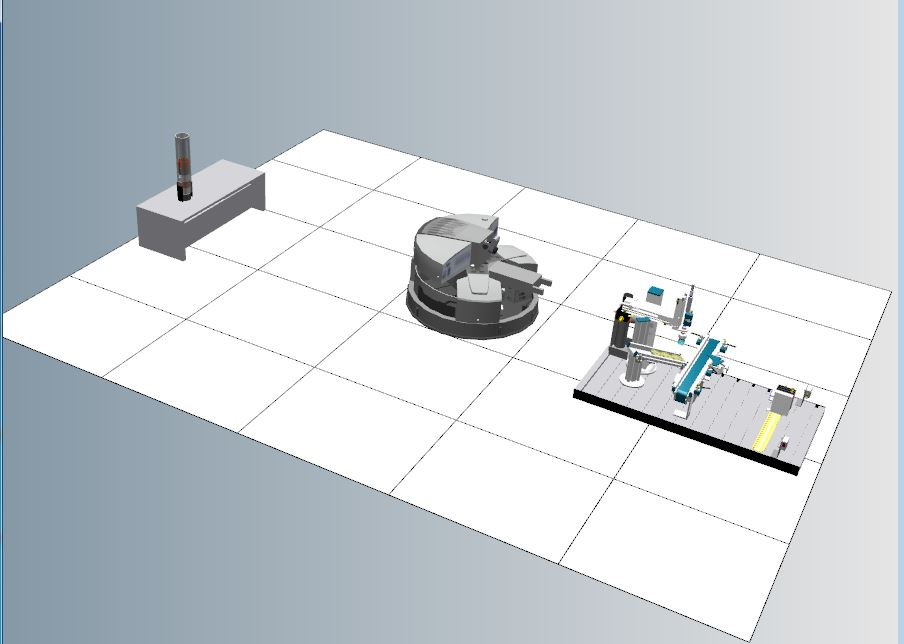
\includegraphics[height=6cm]{MPSDemo.jpg}
  \end{minipage}
} 
\quad
\subfigure[Selection of MPS workpieces]{%
  \label{fig:workpiece}%
  \begin{minipage}[b]{0.3\linewidth}
    \centering
    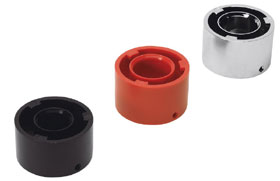
\includegraphics[height=2.5cm]{selectionofworkpieces.jpg}
    \vspace*{2cm}
  \end{minipage}
}
\caption{Approaching an MPS station: The challenge scenario and used workpieces}
\label{fig:mps-challenge}
\end{figure}

\paragraph{Workpiece.~}
The workpieces are round objects with a diameter of
\SI{40}{\milli\metre} and are of red, black, or silver color. They are
made of plastic, cf. \reffig{fig:workpiece}. The team can choose any
of the workpieces.

\paragraph{MPS station}
The MPS station is mounted on a rectangular profile plate of size
\SI{350}{\milli\metre} $\times$ \SI{700}{\milli\metre} with a height
of \SI{30}{\milli\metre}. The transfer points (MPS and shelf) are
\SI{148.165}{\milli\metre} above ground, the workpiece has to be
lifted completely above this height. The transfer point is the center
of the conveyor belt. Relative to long side of the base plate it is
located \SI{375}{\milli\metre} from one side and
\SI{325}{\milli\metre} from the other. The belt has a width of
\SI{45}{\milli\metre} and is at the transfer point height. With this
information teams can create a mockup of this machine for training and
development of custom manipulation devices.

\begin{figure}[h]
\centering
\subfigure[Overview Pick \& Place]{%
  \label{fig:mps-overview}%
  \begin{minipage}[b]{0.45\linewidth}
    \centering
    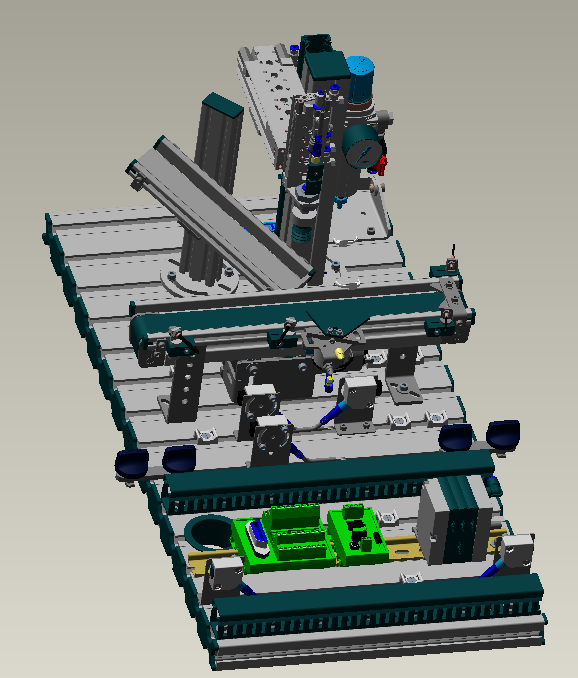
\includegraphics[height=7cm]{mps_overview.png}
  \end{minipage}
} 
\quad
\subfigure[Interface point height]{%
  \label{fig:mps-docking}%
  \begin{minipage}[b]{0.45\linewidth}
    \centering
    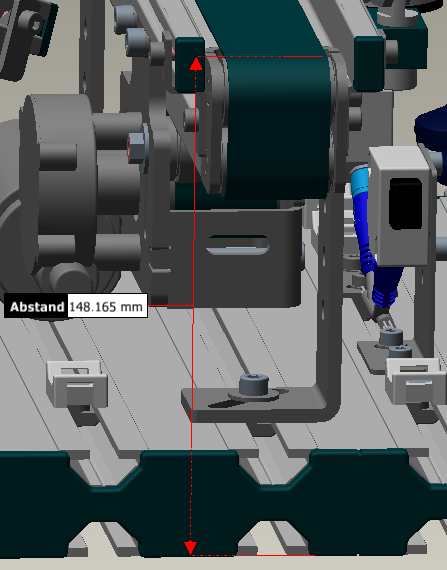
\includegraphics[height=7cm]{mps_docking.png}
  \end{minipage}
}
\caption{The MPS station in detail}
\label{fig:mps-station}
\end{figure}

\subsubsection{Free challenge~}
Each team will be given 5 minutes to showcase their robot team, e.g.
show some new robotics developments. This may involve any task as long
as it is performed with at most three Robotino robots within the
competition area. For the time of the free challenge, any software or
hardware modification is allowed, even though otherwise disallowed in
the regular competition. This may be used to showcase ideas for future
developments of the league and to highlight particular advances in the
system of the presenting team.

The team leaders of non-presenting team will judge the performance and
rate it with points between 0--10.  The team with the highest sum of
points will win this challenge. The other teams are ranked in
decreasing point order.

\subsubsection{Conducting the Challenges~}
The technical challenges are conducted in the following way. The team
leaders of each participating team agree on a date and time during the
tournament for the Technical Challenge in their first team leader
meeting. For each type of challenge, a time slot is assigned, in which
teams can participate once in the challenge. Each team can register
for any of the challenges. All team leaders have to be present at the
time of the challenge to judge the other teams. The OC is responsible
to conduct the Technical Challenge and can appoint team leaders as
support. Each challenge will have a separate ranking. In each ranking,
the team on the last rank will receive 0 points, the last-but-one
ranked team will receive 1 point etc. The points for each ranking will
be added and the team with the most points accrued over all challenges
will be awarded with the Logistic Leagues Technical Challenge Award.


\section{The Robotino System}
\label{sec:robotino}

All participants have to design their competition Robotinos within the
following specifications. For a detailed technical description of the
basic hardware, refer to the Appendix~\ref{sec:engref}. Robotino 2 is
still allowed, however, we strongly recommend using the Robotino 3 as 
the robot hardware platform from this year on.

Any kind of sensors can be changed or added to	 the Robotino platform.
However, it is not possible to implement sensors that require 
modifications outside the Robotino area (e.g. Northstar, indoor GPS).
There must be no changes to the controller or mechanical system.
The robots peripherals must not exceed the maximum total height of 
\SI{1.1}{\metre} including the tower and the table on top. Additional
hardware (sensors, computing equipment, etc.)  must be within a circle 
of a diameter of \SI{0.65}{\metre}  (for both, Robotino 2 and 3) or 
centered at the robot's rotational center-point. Additional hardware 
may only occupy up to $25\%$ of this additional \SI{0.14}{\metre} 
(Robotino 2) or \SI{0.10}{\metre} (Robotino 3) wide ring around the 
robot. The only additional actuator allowed is one gripping device for 
workpieces which can be the original or a modified one. It also must 
be within the same diameter of the other additional hardware. The 
gripper is allowed to transport one workpiece at a time. And the 
gripper must release the workpiece for safety whenever the referee 
wants to take out it. For example, if the referee presses the release 
button or key, the gripper releases the workpiece.

It is allowed to install additional computing power on the
\Robotino. This may either be in form of a notebook/laptop device or
any other computing device that suits the size requirement of the
\Robotino{} competition system. Furthermore, it is allowed to
communicate with an additional computing device off-field. This device
may be used for team coordination and/or other purposes. However,
communication among the robots and the off-field device is not
guaranteed during the competition.

\subsection{Markings}
\label{sec:robot-markings}
All field robots must be assigned a single unique number out of the
set $\{1, 2, 3\}$. The number must be written on the robot in one or
more places and clearly visible from all directions, e.g. printed
adhesive labels placed on top or the sides of the robot. The number
must be the same as is announced in the beacon signal to the referee
box (cf.~\refsec{sec:referee-box}).

For audiences and observers to distinguish both teams, all robots must 
wear their respective unique colored label which is either cyan or magenta. 
The Velcro will be provided and is suggested to be placed on the tower's side 
of each robot, the actual color-coded rings are then dynamically divided among 
the playing teams.

\section{Communication}
\label{sec:communication}

Robots have to operate autonomously, that is, without any human
interference during the game. Communication among robots and to
off-board computing units is allowed only using wifi
(cf.~\refsec{sec:wifi-regulations}). Communication is not guaranteed
and may be unavailable during parts of the game. Interruptions must be
expected and are no reason to pause or abort a game, even if they
endure for long periods of the game.

\subsection{Bandwidth Allocation}
\label{sec:bandwidth}
No minimum bandwidth is guaranteed. The amount of communicated data
over the wifi connection shall not exceed
\SI[per-mode=symbol]{2}{\mega\bit\per\second}. Even though the lower
layers could provide for more bandwidth, the overall available
frequency spectrum and wifi channels have to be shared, not only
within our own league. Generally, a conservative use of bandwidth
resources is advised. Should a frequently or endured exceedance of the
bandwidth limit become known, or if the overall bandwidth limit must
be reduced due to outer circumstances, the TC can monitor the network
traffic and demand reduction in communicated data as necessary.

\subsection{Referee Box (refbox)}
\label{sec:referee-box}
The referee box (refbox) is a software system that runs on a system
provided by the Organization Committee. It controls the overall game,
monitors feedback from the robots, and awards points. It is instructed
by an assisting human referee and keeps a log of all relevant game
events. The final game report will be produced by the referee
box. While we strive for a maximum of automation of this control task,
we rely on the human referee for final judgment, in particular for
border or under-specified cases, and will provide the largest set of
override abilities feasible.

The refbox is the single point of instruction for robots during the
game. After game setup has finished, game state information and orders
are announced by the refbox. Commands must be acknowledged. In certain
situations (for example during the exploration phase) for successful
and true communication with the refbox points are awarded. The aim is
to reduce human interference year by year to a minimum as to exhibit
the widest autonomy during the game possible. Ultimately, the refbox
should be able to fully control the game by itself, transforming all
participants, team members, and visitors alike into pure spectators of
the game, sometimes providing maintenance and crisis intervention when
necessary.

The communication from the refbox to the robot is a datagram-oriented
broadcast protocol based on Google protocol buffers\footnote{Available
  at \url{https://code.google.com/p/protobuf/}} (protobuf). The
protocol definition and technical parameters are described in detail
in the RoboCup Logistics League Referee Box Integrator's
Manual~\cite{RefBoxIntManual}

\subsection{Remote Control}
\label{sec:remote-control}
Remote operation or instruction of any kind of the robots is forbidden
at all times during a game. The only allowed interaction is for the
start-up (cf.~\refsec{sec:game-start}). Any failure to comply with
this rule will lead to immediate disqualification of the infringing
team.

\subsection{Monitoring}
\label{sec:monitoring}
\emph{Passive} monitoring, i.e. receive-only communication from a base
station of the robots' performance is allowed. However, the overall
bandwidth limit may not be exceeded.
%, this includes in particular, but
%is not limited to, images and other raw data.
If the referee has any reason to belief that a monitoring application
might be used for instruction, he can demand the shutdown of the
monitoring software (also refer to previous section on Remote
Control).

\subsection{Inter-robot Communication}
\label{sec:inter-robot-comm}
Robots currently active on the field can freely exchange any
information that supports a coordinated team play. Robots not actively
participating in the game, for example because they have been
irrevocably removed from the current game, may not communicate with
the other robots. It is forbidden to communicate with any sensors that
are not physically attached to the robot, including, for example, but
not limited to a camera aside the field. Likewise any off-robot
actuator is forbidden.

\subsection{Communication Eavesdropping and Interference}
\label{sec:comm-tampering}
% This might sound harsh, but it's based on lessons learned in
% numerous years of RoboCup, you wouldn't believe what some teams will
% do... :-/
Communication of another team may neither be eavesdropped on nor be
interfered with. Teams not currently active shall disconnect from the
field access points.

Monitoring of bandwidth used or of possible misbehavior may only be
performed by members of the TC or an appointed delegate.
% can add this, need to be clear that this must be done using a team
% leader majority vote and not just any team leader
% or by a person appointed by the team leaders.
Any indication of misbehavior will be discussed by the team leader
convention and may result in penalties or disqualification from the
tournament.


%Each robot has to operate autonomously. The communication between the
%robot and the device responsible for the Start/Stop command, as well
%as all communication amongst the robots has to be realized using the
%Wi-Fi connection. The program controlling the robot has to be executed
%locally by the robot itself. % It is strictly forbidden to use any kind
%% of external server acting as command point.
%\begin{rulechange}
%  The robots will receive their commands from the Referee-Box as
%  specified in the referee box protocol. Further, communication to one
%  dedicated off-board computing device is allowed. However, wifi
%  communication should not taken for granted during competition by the
%  participating teams. 
%\end{rulechange}
%The robots are allowed to share information with other devices, but
%must receive nothing else but the start, pause and stop command
%from units other than the 2 fellow robots. This specifically excludes:
%Usage of processed image data created outside of the robots A central
%communication that requires a device other than the three Robotinos A
%permanently established connection between the command device and the
%Robotinos.

\subsection{Wifi Regulations}
\label{sec:wifi-regulations}
In order to provide the optimal possible solution for wireless
communication during the event, all teams are required to use the
\SI{5}{\giga\hertz} wifi equipment. They are furthermore required to
connect their Robotinos wifi unit to the access point provided. All
teams can also rely on wifi clients supplied by Festo but are not
required to. A detailed description concerning the infrastructure can
be found in Appendix~\ref{sec:wifi-equipment}.

% Please refer to Sect.~\ref{sec:radio-interference} for further details.

%%%%%%%%%%%%%%%%%%%%%%%%%%%%%%%%%%%%%%%%%%%%%%%%%%%%%%%%%%%%%%%%%%%%%%%%%%%%%
%%%


%%%%%%%%%%%%%%%%%%%%%%%%%%%%%%%%%%%%%%%%%%%%%%%%%%%%%%%%%%%%%%%%%%%%%%%%%%%%%
%%%

% \section{Development / Vision}

% This section is meant to enable discussions and support investment
% decisions for future soft- and hardware acquisitions.

% \subsection{Short term ideas}

% These are ideas that could still be incorporated into the rulebook of
% Istanbul 2011. 

% \subsubsection{Scripted, dynamic obstacles}

% On the way to fully dynamic obstacles this iteration implies a fully
% scripted administration controlled Robotino that follows implicit
% movement rules that are known to all participants.

% \subsection{Midterm planning}
% Additions and alterations for future iterations of this competition


% \subsubsection{Various Production programs}
% A part from the three-staged production process, various goods with
% different work orders and specifications (e.g. top speed, delivery
% strategies...) could be part of the challenge. This addition seems to
% be heavily dependent on Sect.~\ref{sec:supp-flow}.

% \subsubsection{Various order strategies}
% A delivery could consist of more than one final product, it could be
% required to deliver a batch of products, maybe within a certain time
% span, to complete the loading and receive extra points. Also, the
% different delivery gates could obtain a predefined shipping list, for
% example gate 1 requiring 2 Products, 2 M2 and 1 M1, maybe in the
% correct order to enable FIFO, LIFO or other delivery strategies.

% \subsubsection{Simulation league}

% Since there is only the annually world championship and maybe a
% regional preregistration, a simulation platform could be provided,
% where the software framework of teams can be used to compete with
% other teams. Additionally a branch of simulation could be created that
% focuses on the simulation of many AGV and a huge production area in
% order to compete on scalability.

% \subsubsection{Introducing a supportive flow of information}
% \label{sec:supp-flow}

% As the current task only deals with the material stream, it is heavily
% limited to a simple static task. In order to enable a flow of
% information that transports complex orders, a combined effort should
% focus on implementing a data interface that can be used by all teams
% today and in the future. As this would be a giant leap towards the
% industrial application, a general discussion and a lot of effort has
% to be invested into this issue.


% \subsection{Long term Vision}
% Ideas, dreams and ideology that inspire the future development.

% \subsubsection{Complex production machines}
% As there are more ways to interact with a machine than mounting and
% dismounting a loading carrier, it is possible to develop new machine
% types that look different and are completely different to handle.

% \subsubsection{Collaborative Production}
% Teams could be required to cooperate with another team to enable a
% combined supply chain. 

% \subsubsection{Opponent controlled dynamic obstacles}
% No scripted obstacle can truly represent challenges of the industrial
% application. In the long run, an opposing team has to be reinserted
% that is allowed and requested to anticipate the logistic processes in
% real time in order to create worst case scenarios for the teams.

% \subsubsection{Interfacing ERP / SCM}
% The interface used to present orders could be back ended with software
% from real business applications like ERP, PPS, WHM and SCM.

% \subsubsection{JIS / JIT implementation}
% With complex production processes and several other achievements and
% upgrades it could be useful to implement JIS and JIT tasks and
% procedures into the LL, requiring delivery strategies like LIFO, FIFO
% and certain time windows.

%%%%%%%%%%%%%%%%%%%%%%%%%%%%%%%%%%%%%%%%%%%%%%%%%%%%%%%%%%%%%%%%%%%%%%%
%%% 

\begin{appendix}
\newpage

\section{Engineering Reference}
\label{sec:engref}
\subsection{The Mobile Robot System Robotino 3}
The mobile robot system Robotino is a platform with open mechanical
and electrical interfaces for the integration of additional devices
like sensors or motors. By default power is supplied via two
exchangeable \SI{12}{\volt} lead gel batteries which permit a running
time of up to two hours. Robotino is driven by 3 independent,
omni-directional drive units. They are mounted at an angle of
\ang{120} to each other. The three omni-directional drive units of
Robotino defines it as being holonomic, meaning that the controllable
degrees of freedom equals the total degrees of freedom of the
robot. The drive units are integrated in a sturdy, laser welded steel
chassis. The chassis is protected by a rubber bumper with integrated
switching sensor.

\subsubsection{Robot Dimensions (w/o extension tower)}
\label{apx:sec:robot}
\begin{itemize}
\item \textbf{Diameter:} \SI{450}{\milli\metre}
\item \textbf{Height including housing:} \SI{290}{\milli\metre}
\item \textbf{Overall weight:} approx. \SI{22.5}{\kilogram}
\item \textbf{Maximal payload:} about \SI{30}{\kilogram}
 \end{itemize}

\subsubsection{Drive Unit}
\begin{itemize}
\item \textbf{3$\times$ omni-directional wheels:} \SI{120}{\milli\metre}
\item \textbf{Fed by DC three motors:} \SI{3600}{rpm}
\item \textbf{Gear transmission ratio 32:1} \SI{22.5}{\kilogram}
 \end{itemize}

\begin{figure}[h]
\centering
\subfigure[Festo Robotino 2]{%
  \label{fig:robotino-2}%
  \begin{minipage}[b]{0.3\linewidth}
    \centering 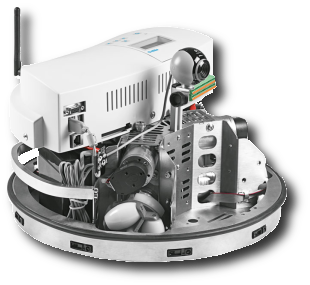
\includegraphics[height=3.5cm]{figures/robotino-shadow}
  \end{minipage}
} 
\quad
\subfigure[Festo Robotino 3]{%
  \label{fig:robotino-3}%
  \begin{minipage}[b]{0.3\linewidth}
    \centering
    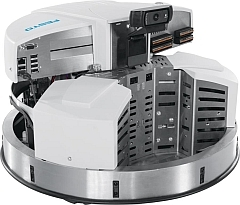
\includegraphics[height=3.5cm]{Robotino3.jpg}
  \end{minipage}
}
\caption{Robotino 2 and Robotino 3 without extension tower}
\label{fig:robotinos}
\end{figure}

\hskip-\parindent The motor speed will be controlled via a PID
controller implemented on a Atmel microprocessor of the controller
board of Robotino.

\subsubsection{Sensors}
Robotino is equipped with 9 vertical mounted infrared distance
measuring sensors which are mounted in the chassis at an angle of
\ang{40} to one another. Robotino can scrutinize all surrounding areas
for objects with these sensors.  Each of the sensors can be queried
individually via the controller board. Obstacles can thus be avoided,
clearances can be maintained and bearings can be taken on a selected
target. The sensors are capable of accurate or relative distance
measurements to objects at distances of \SI{4}{\centi\metre} to
\SI{30}{\centi\metre}. Sensor connection is especially simple
including just one analogue output signal and supply power. The
sensors' evaluation electronics determines distance and read it out as
an analogue signal.  The anti-collision sensor is comprised of a
switching strip which is secured around the entire circumference of
the chassis. A reliably recognizable signal is thus transmitted to the
controller unit.  Collisions with objects at any point on the housing
are detected and, for example, Robotino is brought to a
standstill. The inductive proximity sensor is supplied as an
additional component. It serves to detect metallic objects on the
floor.

The default webcam camera is plugged in via USB and is capable of full
HD 1080p video with auto light correction and two built in microphones
for stereo sound with noise-canceling.

\subsubsection{Controller Board}
Robotino is powered by an exchangeable Embedded PC - COM Express
layout combined with a custom made sensor board.

\paragraph{Embedded PC according to COM Express specification}
\begin{itemize}
\item Embedded Intel Core i5, 2.4 GHz, Dual-Core
\item 8 GB RAM
\item 64 GB SSD (exchangeable) 
\item Operating system: Linux Ubuntu 12.04 (64-bit)
\end{itemize}

\paragraph{Embedded PC interfaces}
\begin{itemize}
\item 1 $\times$ Ethernet
\item 6 $\times$ USB 2.0
\item 2 $\times$ PCI Express expansion slot
\item Wireless LAN according to 802.11b/g, client or access point mode
\item 2 $\times$  RS232
\item 1 $\times$ Parallel port and 1 $\times$ VGA port
\item Wireless LAN Access Point following the standards 802.11/b/g.
\item The access point supports client mode, optional WPA2 encryption.
\end{itemize}

\paragraph{Motor control}
\begin{itemize}
\item micro-controller with 32-bit microprocessor and separated
  Ethernet interface
\item Including 1 $\times$ additional motor output and encoder
  connector
\item 8 $\times$ analog inputs from 0 V to 10 V (50 Hz)
\item 8 $\times$ digital inputs/outputs with 24 V, short circuit proof
  and overload protected
\end{itemize}

\subsubsection{Power supply}
\begin{itemize}
\item 2 $\times$ 12 V lead-fleece rechargeable batteries with 9.5 Ah
  capacity each
\item Operating time(default batteries): up to 4 hours
\item Power supply for additional components: 13 x 24 V, 13 x GND
\item Internal charger for lead-gel and NiMH rechargeable batteries
\item 24 V power supply for charging batteries
\end{itemize}

\subsubsection{Software}
Pre-installed is Ubuntu Linux 12.04 LTS operating system. The main
part of the controller is the Robotino server, a real time Linux
application. It controls the drive units and provides interfaces to
communicate with external PC applications via wifi. Also provided: API
2.0 with libraries which allow you to create applications for Robotino
in numerous programming languages:

\begin{itemize}
\item C++ and C 
\item C\# 
\item .net and JAVA 
\item MatLab and Simulink
\item Labview
\item Robot Operating System (ROS)
\item Microsoft Robotics Developer Studio
\end{itemize}

You may find a lot of examples concerning using the different API's in
the public OpenRobotino forum at \url{http://www.openrobotino.org}.

\paragraph{Webinterface}
HTML5-based user interface provided by webserver running on Embedded
PC for setup and configuration using SmartPhone, Tablet or PC/Notebook
User interface supporting program management, manual control, network
setup, status display and options Help system: online manual for
getting started, details on all components and introduction into
programming

\paragraph{Robotino View} 
For a quick start or Hardware testing there is proprietary drag and
drop Software Robotino View. Graphical programming environment for
external PC running on Windows XP, Vista, Windows 7 or Windows 8.

\begin{itemize}
\item Main program using sequential function chart according to IEC 61131
\item Reusable subprograms based on function blocks
\item Library for function blocks and devices
\item Global variables for communication between subprograms
\item Program interpreter to run programs on Embedded PC autonomously
\end{itemize}

\hskip-\parindent Additional information as well as accessories can be
obtained through\\
\url{http://www.robocup-logistics.org/links/festo-robotino-3}.

\subsection{Robotino 2.0 (phase-out model)}
The mobile robot system Robotino is a platform with an open
mechanical interface for the integration of additional mechanical
devices and an open electrical interface to integrate easily
additional sensors or motors of devices. Power is supplied via two
\SI{12}{\volt} lead gel batteries which permit a running time of up to
two hours.  The scope of delivery likewise includes a charging
device. Robotino is driven by 3 independent, omni-directional drive
units. They are mounted at an angle of \ang{120} to each other. The
three omni-directional drive units of Robotino, defines the robot as
being holonomic, meaning that the controllable degrees of freedom
equals the total degrees of freedom of the robot. The drive units are
integrated in a sturdy, laser welded steel chassis. The chassis is
protected by a rubber bumper with integrated switching sensor.

\subsubsection{Robot Dimensions}\label{apx:sec:robot}
\begin{itemize}
\item \textbf{Diameter:} \SI{370}{\milli\metre}
\item \textbf{Height including housing:} \SI{210}{\milli\metre}
\item \textbf{Overall weight:} approx. \SI{11}{\kilogram}
\item \textbf{Maximal payload:} about \SI{6}{\kilogram}
\end{itemize}

\subsubsection{Drive Unit}
Each of the 3 drive units consists of the following components: DC
Dunker motor with nominal speed of \SI{3600}{rpm} and nominal torque
of \SI{3.8}{\newton\centi\metre}. Integrated planetary gear unit with
a gear ratio of 4:1. Omni-directional wheels of diameter of
\SI{80}{\milli\metre}. Toothed belt with gear wheels providing a
transmission ratio of 4:1. Altogether this provides a gear
transmission ratio of 16:1. Incremental encoder with a resolution of
2048 increments per motor rotation. The motor and gear arrangement is
shown in Figure~\ref{fig:driveunit}.

The motor speed will be controlled via a PID controller implemented on
a Atmel microprocessor of the controller board of Robotino.

\subsubsection{Sensors}
Robotino is equipped with 9 infrared distance measuring sensors which
are mounted in the chassis at an angle of \ang{40} to one
another. Robotino can scrutinize all surrounding areas for objects
with these sensors.  Each of the sensors can be queried individually
via the controller board. Obstacles can thus be avoided, clearances
can be maintained and bearings can be taken on a selected target. The
sensors are capable of accurate or relative distance measurements to
objects at distances of \SI{4}{\centi\metre} to
\SI{30}{\centi\metre}. Sensor connection is especially simple
including just one analogue output signal and supply power. The
sensors' evaluation electronics determines distance and read it out as
an analogue signal.  The anti-collision sensor is comprised of a
switching strip which is secured around the entire circumference of
the chassis. A reliably recognizable signal is thus transmitted to the
controller unit.  Collisions with objects at any point on the housing
are detected and, for example, Robotino is brought to a
standstill. The inductive proximity sensor is supplied as an
additional component. It serves to detect metallic objects on the
floor.

The inductive proximity sensor must be attached to the mounting
furnished for this purpose, and must be connected to the I/O
interface.  The output voltage is \SI{0}{\volt} to \SI{10}{\volt}. The
sensing range is \SI{0}{\milli\metre} to \SI{6}{\milli\metre}. Path
tracking can also be implemented with the two included diffuse
sensors.  Flexible fiber optic cables are connected to a fiber-optics
unit which works with visible red light. Reflected light is
detected. Different surfaces and colors produce different degrees of
reflection. However, gradual differences in reflected light cannot be
detected. The sensors must be attached to the mountings furnished for
this purpose, and must be connected to the I/O interface.

Robotino is equipped with a color webcam. The webcam is equipped with
a USB interface. Also, there will be integrated a digital Gyroscope
providing a high accuracy of the odometry in the virtual factory.

\subsubsection{Controller Board – 2010 Revision}

\begin{figure}[h]
\centering
\subfigure[Drive unit with motor (1), encoder (2), omni-directional wheel (3)]{%
  \label{fig:driveunit}%
  \begin{minipage}[b]{0.4\linewidth}
    \centering 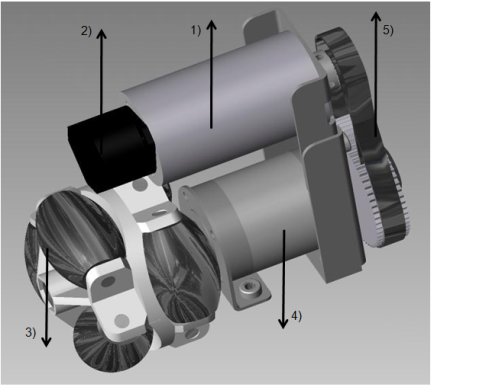
\includegraphics{driveunit.png}
  \end{minipage}
} 
\quad
\subfigure[Festo Robotino 2 inside view]{%
  \label{fig:robotino-2-board}%
  \begin{minipage}[b]{0.45\linewidth}
    \centering
    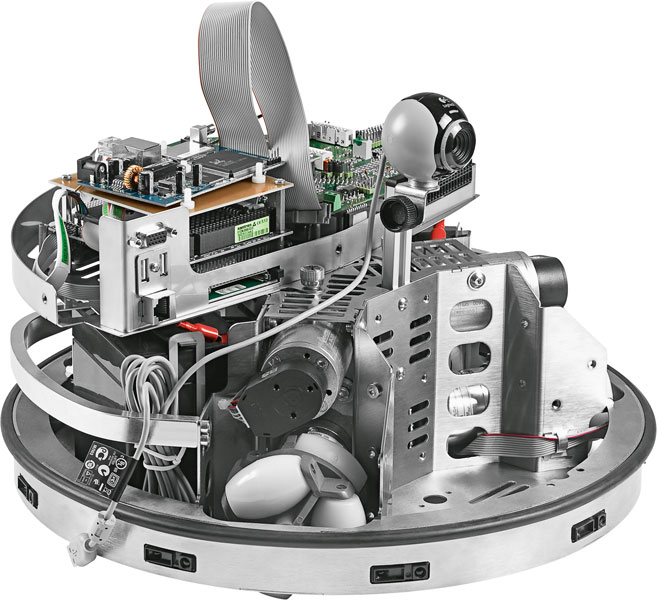
\includegraphics[height=5.5cm]{RobotinoOpen.jpg}
  \end{minipage}
}
\caption{Robotino 2 internals}
\label{fig:robotino-2-guts}
\end{figure}

The controller housing is connected to the wiring in the chassis via
one plug-in. Thus you can easily take off the controller housing and
you have direct access to the mechanical system. The controller system
of Robotino is divided into two parts – an embedded PC and a
micro-controller interface card: The Controller of Robotino consists of
an embedded PC and a micro-controller interface board. The main
controller is the embedded PC 104 plus controller with the 500 MHz
processor AMD LX800. The PC has a SDRAM of 128 MB and is provided with
a 1 GB flash card. There are numerous communication interfaces on
board:

\begin{itemize}
\item 2 $\times$ \SI[per-mode=symbol]{100}{\mega\bit\per\second} Ethernet
\item 2 $\times$ external USB, 1 $\times$ on-board USB-connector
\item 2 $\times$  RS232
\item 1 $\times$ Parallel port and 1 $\times$ VGA port
\item Wireless LAN Access Point following the standards 802.11/b/g.
\item The access point can be switched into a client mode.  As an
  option you may use WPA2-coding.
\end{itemize}

\subsubsection{Software}
Pre-installed is an Ubuntu Linux operating system with real time kernel
running on the embedded PC 104. The main part of the controller is the
Robotino server, a real time Linux application. It controls the drive
units and provides interfaces to communicate with external PC
applications via wifi. There is an API with libraries which allow you
to create applications for Robotino in numerous programming languages:

\begin{itemize}
\item C++ and C 
\item C\# 
\item .net and JAVA 
\item MatLab and Simulink
\item Labview
\end{itemize}

\hskip-\parindent You may find a lot of examples concerning using the
different API's in the public OpenRobotino forum at
\url{http://www.openrobotino.org}.

\paragraph{Robotino View} 

Robotino View is a graphical programming language with numerous
prepared function blocks you can easily connect via input and output
parameters to establish more complicated function diagrams. You can use
these function diagrams as subprograms for more complex programming
sequences. To build up general programming sequences Robotino View
follows the international standard IEC 61131-3. You may run Robotino
View on an external PC and Robotino View communicates directly with
the Robotino Server on the PC 104 via wifi in order to control the
robot system. The function blocks receive a direct feedback of the
hardware components such that you can live interact with the robot
system. On the other hand you can download Robotino View programs into
the PC 104 in order to run the applications completely autonomously.
There is a well defined interface to develop own function blocks in C++
or Lua.

\paragraph{Image Processing}

Depending on the Robotino version it might happen that the standard web
camera only provides image data by JPEG compression. This is very
useful if you run your image processing on the PC and exchange the data
via wifi. However, if you would like to run your image processing
algorithms on the Robotino controller then the processor is not
powerful enough in order to pack and to unpack the image data in a
reasonable time. Thus we recommend for running image processing
algorithms on the Robotino controller to use a camera without JPEG
compression, e.g. use the low cost Logitech web camera C250.

%\subsection{Machines}
%\label{abx:sec:machine}
%
%\begin{figure}[h]
%\centering
%\subfigure[Ranges and dimensions of a signal]{%
%  \label{apx:fig:machinemeasures}%
%  \begin{minipage}[b]{0.45\linewidth}
%    \centering \includegraphics[width=\textwidth]{machine_measures.png}
%  \end{minipage}
%}
%\quad
%\subfigure[Ranges and dimensions of the supporting brackets]{%
%  \label{apx:fig:brackets}%
%  \begin{minipage}[b]{0.45\linewidth}
%    \centering
%    \includegraphics[width=\textwidth]{bracket.png}
%  \end{minipage}
%}
%\caption{Machine Details}
%\label{fig:machine-details}
%\end{figure}
%
%\subsubsection{Signal}
%\begin{table}[H]
%  \centering
%  \mytable{\begin{tabularx}{\linewidth}{l|X}
%      \hline
%      Dimension \&	diameter&	\SI{36}{\milli\metre} \\
%      height(total)		 	&	\SI{147}{\milli\metre} \\
%      Segment height 			&	\SI{34}{\milli\metre},
%      including \SI{5}{\milli\metre} unlighted border \\
%      Lifespan				&	max. \SI{50.000}{\hour} \\
%      Connector				&	Bottom, \SI{2}{\metre} supplied 
%      Compatible to the I/O-Terminal of MPS(r) units. \\
%      Safety					&	IP65 \\
%      Voltage					&	\SI{24}{\volt} \\
%      Current					&	3 $\times$ \SI{40}{\milli\ampere} \\
%      Kind of current			&	DC \\
%      Operating mode			&	\SIrange{-20}{+50}{\degreeCelsius} \\
%      Signal type				&	Static LED \\
%      Signal					&	Ultra-bright LED\\
%      Source					&	Festo \# 549843 \\
%%      \hline
%    \end{tabularx}}
%  \caption{Technical specification of the signal}
%  \label{apx:tab:signalproperties}
%\end{table}
%
%\subsubsection{RFID device}
%
%\begin{table}[H]
%  \centering
%  \mytable{\begin{tabularx}{1\linewidth}{l|X}
%      \hline
%      Technical data of the read/write head		&	Housing rectangular \\
%      Housing and working dimensions 				&
%      \SI{40x40}{\milli\metre}  with the centered RFID
%      tag. \\
%      Housing height
%      & \SI{65}{\milli\metre} \\ 
%      Operating voltage							&	DC \\
%      Housing material Plastic					& 	PBT-GF30-V0, black \\
%      Material active face Plastic				& 	PA6-GF30, yellow \\
%      Operating voltage
%      & 	\SIrange{10}{30}{\volt.DC} \\
%      DC rated operational current				& 	$\le$ \SI{80}{\milli\ampere} \\
%      Data transfer								& 	inductance coupling \\
%      Working frequency							& 	\SI{13.56}{\mega\hertz} \\
%      Radio communication and protocol standards	&	ISO 15693 \\
%      Read/write distance							&	max. \SI{115}{\milli\metre} \\
%      Output function								&	4-wire, read/write \\
%      Electrical connection 						&	Connectors M12 $\times$ 1 \\
%       Vibration resistance						&	\SI{55}{\hertz} (\SI{1} {\milli\metre}) \\
%       Shock resistance							&	\SI{30}{\gram} (\SI{11}{ \milli\second}) \\
%       Protection class							&	IP67 \\
%       Operating voltage display					& 	LED green \\
%% %      \hline
%    \end{tabularx}}
%  \caption{Technical specification of the RFID device}
%  \label{apx:tab:rfidproperties}
%\end{table}

\subsubsection{Wifi equipment}
\label{sec:wifi-equipment}
\begin{table}[H]
  \centering
  \mytable{
    \begin{tabularx}{1\linewidth}{l|X}
      \hline
      Festo AP		&	LANCOM L-322agn \\
      Transfer rate		&	Up to \SI{108}{\mega\bit\per\second} \\
      Data link protocol	&	802.11 a/g/n \\
      Frequency			&	\SI{5.0}{\giga\hertz} \\
      IP-distribution		&	172.26.200.xxx for LAN clients(DHCP) \\
      &	172.26.101.xxx for the Robotino devices \\
      &	172.26.1.xxx for Robotinos \\
      Subnet Mask			&	255.255.0.0 \\
      Encryption			&	Unsecured \\
      SSID				&	Separated for both teams:\\
      &	RobotinoEvent.1 \\
      & RobotinoEvent.2 \\
      Festo Clients		&	3COM WL-560 \\
      Power Supply		&	Clients: \SI{12}{\volt}, \SI{1}{\ampere},\\
      & 	Most Laptops cannot power them \\
      & 	via USB! \\
      Connector			&	Ethernet \\
      
%      \hline
    \end{tabularx} }
    \caption{Technical specification of the wifi equipment}
	\label{apx:tab:wifi}
\end{table}



\printbibliography

\end{appendix}
\end{document}
